\chapter{\chatextprobRepresentation}\label{cha:probRepresentation}

In this chapter we will establish relations between the formalism of tensor networks and basic concepts of probability theory.
We will first understand distributions as tensors and connect their marginalizations and conditionings to the tensor operations of contractions and normations.
Then we discuss independence assumptions as examples of contraction equations, which lead to tensor network decompositions known as graphical models.
We then treat more generic exponential families and investigate their representation as tensor networks.

\red{We investigate two mechanisms to identify tensor network decompositions of probability distributions:
\begin{itemize}
    \item Independence approach: Conditional independence implies representations by markov networks
    \item Computation approach: When there are sufficient statistics providing probabilities, we construct tensor networks decompositions by computation of the statistics.
\end{itemize}
}

\sect{Classical Properties of Distributions}

To start, we first relate classical properties of distributions, such as independent variables, with the tensor network formalism.

\subsect{Probability Tensors}

%% Random Variables: Introduction in Bayesian way by uncertainties
After having discussed how to represent states of factored systems by one-hot encodings, let us now take advantage of these representation by associating properties with these states.
Let there be uncertainties of the assignments $\catindexof{\atomenumerator}$ to the categorical variables $\catvariableof{\atomenumerator}$ of a factored system.
We then understand $\catvariableof{\atomenumerator}$ as random variables, which have a joint distribution defined by the uncertainties of the state assignments.
To capture these uncertainties we now make use of the one-hot representation of factored systems.

\begin{definition}[Probability Tensor]
    \label{def:probabilityDistribution} % From the axioms of Kolmogorov!
    Let there be for each $\catenumeratorin$ a categorical variable $\catvariableof{\catenumerator}$ taking values in $[\catdimof{\atomenumerator}]$.
    A joint probability distribution of these categorical variables is a tensor
    \begin{align*}
        \probat{\catvariableof{0},\ldots,\catvariableof{\atomorder-1}} : \facstates \rightarrow [0,1] \subset \rr
    \end{align*}
    such that
    \begin{align*}
        \contraction{\probat{\catvariableof{0},\ldots,\catvariableof{\atomorder-1}}} = 1 \, .
%		\sum_{\catindices\in\facstates} \probat{\indexedcatvariables} = 1 \, .
    \end{align*}
\end{definition}

%% One-hot Decomposition -> Contraction Equivalences
The probability tensor to the distribution is a tensor
\begin{align*}
    \probwith\in\bigotimes_{\catenumeratorin}\rr^{\catdimof{\atomenumerator}} \, ,
\end{align*}
where we again use the abbreviation $\shortcatvariables$ for the list of variables $\catvariableof{0},\ldots,\catvariableof{\catorder-1}$.
The tensor can be decomposed as the sum (see \lemref{lem:tensorBasisDecomposition} in \parref{par:three} for more details)
\begin{align*}
    \probwith = \sum_{\shortcatindices\in\facstates} \probat{\indexedshortcatvariables} \cdot \onehotmapofat{\shortcatindices}{\shortcatvariables} \, ,
\end{align*}
where we understand $\probat{\indexedshortcatvariables}$ as the probability of the categorical variables to take the state $\shortcatindices\in\facstates$.
%% Normation condition by Kolmogorovs second axiom
The normation condition $1=\contraction{\probwith}$ has a more convenient equivalence by the coordinate sum
\begin{align*}
    1 = \contraction{\probwith}
    =  \sum_{\shortcatindices\in\facstates}\probat{\indexedshortcatvariables} \, ,
\end{align*}
and thus ensures that all probabilities sum to $1$, which is necessary for the probabilistic interpretation.
While the assumptions of non-negative coordinates in \defref{def:probabilityDistribution} reflects the first probability axiom of Kolmogorov, the assumption of contraction $1$ implements the second axiom (see for example \cite{degroot_probability_2016}).
Since probability distributions contract to $1$, they are directed (see \defref{def:directed}) with all distributed variables outgoing and empty incoming variables (see \figref{fig:probabilityTensor}).

\begin{figure}[hbt!]
    \begin{center}
        \begin{tikzpicture}[scale=0.35,thick] % , baseline = -3.5pt

    \node[anchor=center] (text) at (-2,0) {$a)$};

    \node [circle, draw, thick, fill=gray!50, minimum size = \nodeminsize] (P1) at (0,-3) {\tiny $\catvariableof{0}$};
    \node [circle, draw, thick, fill=gray!50, minimum size = \nodeminsize] (P2) at (3,-3) {\tiny $\catvariableof{1}$};

    \node[anchor=center] (text) at (6,-3) {$\cdots$};

    \node [circle, draw, thick, fill=gray!50, minimum size = \nodeminsize] (P3) at (9,-3) {};

    \node[anchor=center] (text) at (9,-3) {\tiny $\catvariableof{\atomorder-1}$};


    \draw[->]
    (4.5,0) to[bend right=25] (P1);
    \draw[->]
    (4.5,0) to[bend right=10] (P2);
    \draw[->]
    (4.5,0) to[bend right=-25] (P3);

    \node[anchor=center] (text) at (4.5,0.5) {$\edge$};


    \begin{scope}
        [shift={(20,0)}]

        \node[anchor=center] (text) at (-2,0) {$b)$};

        \draw (-1,-1) rectangle (5,-3);
        \node[anchor=center] (text) at (2,-2) {\small $\probtensor$};
%\draw[->] (0,-3)--(0,-5) node[midway,left] {\tiny $\catvariableof{0}$};
%\draw[->] (1.5,-3)--(1.5,-5) node[midway,left] {\tiny $\catvariableof{1}$};
        \node[anchor=center] (text) at (3,-4) {$\cdots$};
%\draw[->] (4,-3)--(4,-5) node[midway,right] {\tiny $\catvariableof{\atomorder-1}$};


        \draw[midarrow]  (0,-3) -- (0,-5) node[midway,left] {\tiny $\catvariableof{0}$};
        \draw[midarrow]
        (1.5,-3)--(1.5,-5) node[midway,left] {\tiny $\catvariableof{1}$};
        \draw[midarrow]
        (4,-3)--(4,-5) node[midway,right] {\tiny $\catvariableof{\atomorder-1}$};
    \end{scope}


\end{tikzpicture}
    \end{center}
    \caption{Probability distributions of variables $\catvariableof{0},\ldots,\catvariableof{\atomorder-1}$, sketched
    a) by a directed edge $\edge$ with all variables outgoing, which is decorated b) by a directed tensor $\probwith$.}\label{fig:probabilityTensor}
\end{figure}


\subsect{Base measures}

From a measure theoretic perspective, probabilities are measurable functions called probability densities, which integrals are $1$ (see for example \cite{degroot_probability_2016}). % Add citations?
In our case of finite dimensional state spaces of factored systems, we implicitly used the trivial tensor $\onesat{\shortcatvariables}$ as a base measure, which measures subsets of states by their cardinality and is therefore refered to as state counting base measure.
The distribution tensors $\probwith$ can then be understood as probability densities with respect to this state counting base measure.
We in this work will also consider more general base measures $\basemeasurewith$, which we restrict to be boolean, that is $\basemeasureat{\indexedshortcatvariables}\in\ozset$ for all states $\shortcatindices$.
When understanding $\probwith$ as a probability density with respect to $\basemeasurewith$, any probabilistic interpretation will be through the contraction $\contractionof{\probwith,\basemeasurewith}{\shortcatvariables}$ and the normation condition reads as
\begin{align*}
    \contraction{\probwith,\basemeasurewith} = 1 \, .
\end{align*}
Since we restrict to boolean base measures, the contraction effectively manipulates the tensor $\probtensor$ by setting the coordinates $\probat{\indexedshortcatvariables}$ to zero, when $\basemeasureat{\indexedshortcatvariables}=0$.
Therefore, multiple tensors $\probtensor$ will have the same proabilistic interpretation, when $\basemeasurewith\neq\onesat{\shortcatvariables}$.
To avoid this ambiguity, we introduce the notation of representability with respect to a base measure $\basemeasure$, by demanding that such coordinates are zero.

\begin{definition}
    \label{def:representationBaseMeasure}
    We say that a probability distribution $\probtensor$ is representable with respect to a boolean base measure $\basemeasure$, if for all $\shortcatindices$ with $\basemeasureat{\indexedshortcatvariables}=0$ we have $\probat{\indexedshortcatvariables}=0$.
    We denote the set of by $\basemeasure$ representable distributions by $\bmrealprobof{\basemeasure}$.
\end{definition}

When a probability distribution $\probtensor$ is representable with respect to a boolean base measure $\basemeasure$, we have the invariance
\begin{align*}
    \probwith=\contractionof{\probwith,\basemeasurewith}{\shortcatvariables}
\end{align*}
and can therefore safely ignore the base measures.
This enables the characterization of by $\basemeasure$ representable distributions by
\begin{align*}
    \bmrealprobof{\basemeasure}
    = \left\{ \probat{\shortcatvariables} \, : \, \uniquantwrtof{\shortcatindicesin}{\probat{\indexedshortcatvariables}\geq0}, \, \contractionof{\probwith,\basemeasurewith}{\shortcatvariables}
    = \probwith \right\} \, .
\end{align*}

Starting with \charef{cha:logicalRepresentation} we will further investigate boolean tensors and relate them with propositional formulas.
In \charef{cha:logicalReasoning} we will connect the representation and positivity with respect to boolean base measures with the formalism of entailment.
The notation $\bmrealprobof{\basemeasure}$ of by $\basemeasure$ representable distributions will later in \charef{cha:networkRepresentation} relate to minterm exponential families introduced therein.

% Positive distribution
We now investigate, which base measures $\basemeasure$ can be chosen for a probability distribution $\probtensor$, such that $\probtensor$ is representable by $\basemeasure$.
Here we want to find a $\basemeasure$, which is in a sense to be defined minimal amount the base measures, such that $\probtensor$ is representable with respect to them.
For this minimality criterion we will develop in \charef{cha:logicalReasoning} orders based on entailment and show the minimality in \theref{the:minimalRepPosBaseMeasure}.
Here, we just introduce the minimality criterion as positivity of a distribution with respect to a base measure.

\begin{definition}
    \label{def:positivityBaseMeasure}
    We say that a probability distribution $\probwith$ is positive with respect to a boolean base measure $\basemeasurewith$, if the distribution is representable by $\basemeasure$ (i.e. $\contraction{\probtensor,\basemeasure}=1$) and for all $\shortcatindices$ with $\basemeasureat{\indexedcatvariables}=1$ we have $\probat{\indexedcatvariables}>0$.
\end{definition}

%This is a slide abuse of the measure theoretic approach to probability theory, since typically the base measure needs to be defined before considering probability distributions. 


\subsect{Marginal Distribution}

Contractions of probability distributions are related to marginalizations as we introduce next.

\begin{definition}[Marginal Probability]
    \label{def:marginalProbability}
    Given a distribution $\probat{\exrandom,\secexrandom}$ of the categorical variables $\exrandom$ and $\secexrandom$ the marginal distribution of the categorical variable $\exrandom$ is defined for each $\exrandind$ as the tensor
    \begin{align*}
        \probat{\exrandom} : [\exranddim] \rightarrow \rr
    \end{align*}
    defined by the contraction
    \begin{align*}
        \probat{\exrandom}
        = \contractionof{\probat{\exrandom,\secexrandom}}{\exrandom} \, .
%		= \sum_{\secexrandindin} \probat{\indexedexrandom,\indexedsecexrandom} \, .
    \end{align*}
\end{definition}

To connect with a more standard defining equation of marginal distributions, let us notice that for any $\exrandindin$
\begin{align*}
    \probat{\indexedexrandom}
    = \contractionof{\probat{\exrandom,\secexrandom}}{\indexedexrandom}
    = \sum_{\secexrandindin} \probat{\indexedexrandom,\indexedsecexrandom} \, .
\end{align*}
Thus, each coordinate of the marginal distribution is the sum of the joint probability of compatible states.
We say that the variable $\secexrandom$ is marginalized out, when building the marginal distribution $\probat{\exrandom}$ of $\exrandom$.
Let us now justify this terminology and show, that any marginal distribution is a probability distribution as introduced in \defref{def:probabilityDistribution}.

\begin{theorem}
    \label{the:marginalContraction}
    Any marginal distribution is a probability distribution.
\end{theorem}
\begin{proof}
    We further have that any marginal distribution is normed, since by the commutativity of contractions (see for more details \theref{the:splittingContractions} in \parref{par:three})
    \begin{align*}
        \contraction{\probat{\exrandom}} = \contraction{\contractionof{\probat{\exrandom,\secexrandom}}{\exrandom}} = \contraction{\probat{\exrandom,\secexrandom}} = 1 \, .
    \end{align*}
    Further any coordinate is non-negative, since it is a sum of non-negative coordinates.
    It follows from \defref{def:probabilityDistribution}, that any marginal distribution is a probability distribution.
\end{proof}

% Diagrammatic representation
In a tensor network diagram we often represent variables $\secexrandom$ not appearing as open variables of a contraction as contracted with the trivial tensor $\onesat{\secexrandom}$.
Following this notation, we depict the marginal distribution in \defref{def:marginalDistribution} by
\begin{center}
    \begin{tikzpicture}[scale=0.3,thick] % , baseline = -3.5pt

\draw (-19,-1) rectangle (-15,-3);
\node[anchor=center] (text) at (-17,-2) {\small $\margprobat{\exrandom}$};
\draw[midarrow]  (-17,-3)--(-17,-5) node[midway,left] {\tiny $\exrandom$}; 

\node[anchor=center] (text) at (-13,-2) {${=}$};

\draw (-11,-1) rectangle (-5,-3);
\node[anchor=center] (text) at (-8,-2) {\small $\probat{\exrandom,\secexrandom}$};
\draw[midarrow]  (-10,-3)--(-10,-5) node[midway,left] {\tiny $\exrandom$}; 
\draw[midarrow]  (-6,-3)--(-6,-5) node[midway,left] {\tiny $\secexrandom$};
\draw (-7,-5) rectangle (-5,-7); 
\node[anchor=center] (text) at (-6,-6) {$\ones$};

\end{tikzpicture}
\end{center}
Since we have shown, that marginal distributions are themself probability distributions, they inherit the outgoing directionality in tensor network diagrams.

% Sets of variables
We notice, that \defref{def:marginalProbability} generalizes to marginalizations of arbitrary sets of variables, when having a distribution $\probat{\shortcatvariables}$ of an arbitrary number of categorical variables.
It suffices for this to interpret $\exrandom$ and $\secexrandom$ as collections of variables, which indices take the states of the respective factored systems.

\subsect{Conditional Probabilities}

Normations of probability distributions result in conditional distributions as we define next.

\begin{definition}[Conditional Probability]
    \label{def:conditionalProbability}
    Let $\probat{\exrandom,\secexrandom}$ be a distribution of the categorical variables $\exrandom$ and $\secexrandom$, such that $\probat{\exrandom,\secexrandom}$ is normable on $\{\secexrandom\}$.
    Then the distribution of $\exrandom$ conditioned on $\secexrandom$ is defined by
    \begin{align*}
        \condprobof{\exrandom}{\secexrandom}
        = \normationofwrt{\probat{\exrandom,\secexrandom}}{\exrandom}{\secexrandom} \, .
    \end{align*}
\end{definition}

\begin{figure}[hbt!]
    \begin{center}
        \begin{tikzpicture}[scale=0.3,thick] % , baseline = -3.5pt


    \node[anchor=center] (text) at (-2,0) {$a)$};

    \node [circle, draw, thick, fill=gray!50, minimum size = \nodeminsize] (P1) at (0,-3) {\tiny $\exrandom$};
    \node [circle, draw, thick, fill=gray!50, minimum size = \nodeminsize] (P3) at (9,-3) {};

    \node[anchor=center] (text) at (9,-3) {\tiny $\secexrandom$};

    \draw[->]
    (4.5,0) to[bend right=25] (P1);
    \draw[<-]
    (4.5,0) to[bend right=-25] (P3);

    \node[anchor=center] (text) at (4.5,0.5) {$\edge$};

    \begin{scope}
        [shift={(43,0)}]

        \node[anchor=center] (text) at (-23,0) {$b)$};

        \draw (-21,-1) rectangle (-15,-3);
        \node[anchor=center] (text) at (-18,-2) {\small $\condprobof{\exrandom}{\secexrandom}$};
        \draw[->]  (-20,-3)--(-20,-5) node[midway,left] {\tiny $\exrandom$};
        \draw[<-]  (-16,-3)--(-16,-5) node[midway,left] {\tiny $\secexrandom$};

    \end{scope}

\end{tikzpicture}
    \end{center}
    \caption{Depiction of conditional probability distributions a) by an edge with the incoming variable $\secexrandom$ and the outgoing variable $\secexrandom$, which is decorated by b) the directed tensor $\condprobof{\exrandom}{\secexrandom}$. }
    \label{fig:conditionalDistribution}
\end{figure}

Since conditional probabilities are normations of probability tensors, they are directed and therefore depicted by directed hyperedges (see \figref{fig:conditionalDistribution}).
For any $\secexrandindin$ we depict the slice $\condprobof{\exrandom}{\indexedsecexrandom}$ defined by a normation operation as
\begin{center}
    \begin{tikzpicture}[scale=0.3, thick] % , baseline = -3.5pt

    \begin{scope}
        [shift={(-13,0)}]

        \draw (-22,-1) rectangle (-14,-3);
        \node[anchor=center] (text) at (-18,-2) {\corelabelsize $\condprobof{\exrandom}{\indexedsecexrandom}$};
        \draw[->-]  (-18,-3)--(-18,-5) node[midway,left] {\colorlabelsize $\exrandom$};

        \node[anchor=center] (text) at (-12,-2) {${=}$};

    \end{scope}

    \begin{scope}
        [shift={(-1,0)}]

        \draw (-21,-1) rectangle (-15,-3);
        \node[anchor=center] (text) at (-18,-2) {\corelabelsize $\condprobof{\exrandom}{\secexrandom}$};
        \draw[->-]  (-20,-3)--(-20,-5) node[midway,left] {\colorlabelsize $\exrandom$};

        \draw[-<-]  (-16,-3)--(-16,-5) node[midway,left] {\colorlabelsize $\secexrandom$};
        \draw[] (-15,-5) rectangle (-17,-7);
        \node[anchor=center] (text) at (-16,-6) {\corelabelsize $\onehotmapof{\secexrandind}$};

        \node[anchor=center] (text) at (-13,-2) {${=}$};
    \end{scope}

    \begin{scope}
        [shift={(0,6)}]

        \draw (-11,-1) rectangle (-5,-3);
        \node[anchor=center] (text) at (-8,-2) {\corelabelsize $\probat{\exrandom,\secexrandom}$};
        \draw[->-]  (-10,-3)--(-10,-5) node[midway,left] {\colorlabelsize $\exrandom$};
        \draw[->-]  (-6,-3)--(-6,-5) node[midway,left] {\colorlabelsize $\secexrandom$};
        \draw[] (-7,-5) rectangle (-5,-7);
        \node[anchor=center] (text) at (-6,-6) {\corelabelsize $\onehotmapof{\secexrandind}$};

    \end{scope}

    \draw (-12,-2) -- (-4,-2);

    \begin{scope}
        [shift={(0,-2)}]

        \draw (-11,-1) rectangle (-5,-3);
        \node[anchor=center] (text) at (-8,-2) {\corelabelsize $\probat{\exrandom,\secexrandom}$};
        \draw[->-]  (-10,-3)--(-10,-5) node[midway,left] {\colorlabelsize $\exrandom$};
        \draw (-11,-5) rectangle (-9,-7);
        \node[anchor=center] (text) at (-10,-6) {$\ones$};
        \draw[->-]  (-6,-3)--(-6,-5) node[midway,left] {\colorlabelsize $\secexrandom$};
        \draw[] (-7,-5) rectangle (-5,-7);
        \node[anchor=center] (text) at (-6,-6) {\corelabelsize $\onehotmapof{\secexrandind}$};

        \node[anchor=center] (text) at (-4,-6) {$.$};
    \end{scope}


\end{tikzpicture}
\end{center}

As we have done before for marginal distribution, we relate \defref{def:conditionalProbability} with a more convenient coordinatewise definition of conditional probababilities.
For any indices $\exrandindin$ and $\secexrandindin$ we have
\begin{align*}
    \condprobof{\indexedexrandom}{\indexedsecexrandom}
    = \frac{\probat{\indexedexrandom,\indexedsecexrandom}}{\contractionof{\probat{\exrandom,\secexrandom}}{\indexedsecexrandom}}
    = \frac{\probat{\indexedexrandom,\indexedsecexrandom}}{\sum_{\exrandindin} \probat{\indexedexrandom,\indexedsecexrandom}} \, .
\end{align*}
The distribution of $\exrandom$ conditioned on $\secexrandom$ is the normed collection of slice of the probability distribution $\probat{\exrandom,\secexrandom}$.
Each slice of the conditioned distribution with respect to incoming variables is a probability distribution itself, as we show next.

\begin{theorem}
    \label{the:conditionalContraction}
    For any $\secexrandindin$ the tensor $\condprobof{\exrandom}{\indexedsecexrandom}$ is a probability tensor.
\end{theorem}
\begin{proof}
    As a normation of a non-negative tensor, the conditional probability $\condprobof{\exrandom}{\indexedsecexrandom}$ and any of its slices is also a non-negative tensor.
    Further, we have for any $\secexrandindin$
    \begin{align*}
        \contraction{\condprobof{\exrandom}{\indexedsecexrandom}}
        & = \sum_{\exrandindin} \condprobof{\indexedexrandom}{\indexedsecexrandom} \\
        &= \frac{\sum_{\exrandindin}\probat{\indexedexrandom,\indexedsecexrandom}}{\sum_{\exrandindin}\probat{\indexedexrandom,\indexedsecexrandom}} \\
        &= 1 \, ,
    \end{align*}
    and therefore each slice is normed.
    We can visualize this calculation exploiting our diagramatic notation as
    \begin{center}
        \begin{tikzpicture}[scale=0.3,thick] % , baseline = -3.5pt

\node[anchor=center] (text) at (-30,-2) {\small $\sum_{\atomlegindexof{\exrandom}} \, \condprobof{X=\atomlegindexof{\exrandom}}{Y=\atomlegindexof{\secexrandom}} \quad {=}$};

\draw (-21,-1) rectangle (-15,-3);
\node[anchor=center] (text) at (-18,-2) {\small $\condprobof{X}{Y}$};
\draw[->]  (-20,-3)--(-20,-5) node[midway,left] {\tiny $X$}; 

\draw[<-]  (-16,-3)--(-16,-5) node[midway,left] {\tiny $Y$}; 
\draw[] (-15,-5) rectangle (-17,-7); 
\node[anchor=center] (text) at (-16,-6) {\small $\onehotmapof{\catindexof{Y}}$};

\draw (-21,-5) rectangle (-19,-7); 
\node[anchor=center] (text) at (-20,-6) {$\ones$};

\node[anchor=center] (text) at (-13,-2) {${=}$};


\begin{scope}[shift={(0,6)}]

\draw (-11,-1) rectangle (-5,-3);
\node[anchor=center] (text) at (-8,-2) {\small $\probof{X,Y}$};
\draw[->]  (-10,-3)--(-10,-5) node[midway,left] {\tiny $X$}; 
\draw (-11,-5) rectangle (-9,-7); 
\node[anchor=center] (text) at (-10,-6) {$\ones$};
\draw[->]  (-6,-3)--(-6,-5) node[midway,left] {\tiny $Y$};
\draw[] (-7,-5) rectangle (-5,-7); 
\node[anchor=center] (text) at (-6,-6) {\small $\onehotmapof{\catindexof{Y}}$};

\end{scope}

\draw (-12,-2) -- (-4,-2);

\begin{scope}[shift={(0,-2)}]

\draw (-11,-1) rectangle (-5,-3);
\node[anchor=center] (text) at (-8,-2) {\small $\probof{X,Y}$};
\draw[->]  (-10,-3)--(-10,-5) node[midway,left] {\tiny $X$}; 
\draw (-11,-5) rectangle (-9,-7); 
\node[anchor=center] (text) at (-10,-6) {$\ones$};
\draw[->]  (-6,-3)--(-6,-5) node[midway,left] {\tiny $Y$};
\draw[] (-7,-5) rectangle (-5,-7); 
\node[anchor=center] (text) at (-6,-6) {\small $\onehotmapof{\catindexof{Y}}$};

\end{scope}

%\node[anchor=center] (text) at (-3,-2) {${=}$};
%
%\draw (-1,-3) rectangle (1,-1); 
%\node[anchor=center] (text) at (0,-2) {$\ones$};
%\draw[<-]  (0,-3)--(0,-5) node[midway,left] {\tiny $Y$};
%\draw[] (-1,-5) rectangle (1,-7); 
%\node[anchor=center] (text) at (0,-6) {\small $\onehotmapof{\catindexof{Y}}$};

\node[anchor=center] (text) at (-1,-2) {${=}\quad 1 \, .$};

%\node[anchor=center] (text) at (9,-7) {${.}$};

\end{tikzpicture}
    \end{center}
    Since for any $\secexrandindin$ the slice $\condprobof{\exrandom}{\indexedsecexrandom}$ is non-negative and contracts to $1$, we conclude that it is a probability distribution.
\end{proof}

We further show, that exactly the directed tensors with non-negative coordinates are conditional probability tensors.

\begin{theorem}
    \label{the:conditionalDirected}
    Any tensor with non-negative coordinates is a conditional distribution tensor, if and only if it is directed with the condition variables incoming and the other outgoing.
\end{theorem}
\begin{proof}
    \proofrightsymbol:
    By \theref{the:conditionalContraction} a conditional probability tensor $\condprobof{\exrandom}{\secexrandom}$ is the normation of a tensor and by \theref{the:normationDirected} a directed tensor.
    Since probability tensors have only non-negative coordinates, their contractions with one-hot encodings also have only non-negative coordinates and also their normations.

    \proofleftsymbol:
    Conversely, let $\hypercoreat{\nodevariables}$ be a directed tensor with $\innodes$ incoming and $\outnodes$ outgoing and non-negative coordinates.
    Then
    \begin{align}
        \probat{\nodevariables} = \frac{1}{\prod_{\node\in\innodes}\catdimof{\node}} \cdot \hypercoreat{\nodevariables}
    \end{align}
    is a probability tensor, since
    \begin{align*}
        \sum_{\atomlegindexof{\innodes}} \sum_{\atomlegindexof{\outnodes}} \probat{\indexedcatvariableof{\nodes}} =
        \sum_{\atomlegindexof{\innodes}} \sum_{\atomlegindexof{\outnodes}} \frac{1}{\prod_{\node\in\innodes}\catdimof{\node}} \cdot \hypercoreat{\indexedcatvariableof{\nodes}} =
        \sum_{\atomlegindexof{\innodes}} \frac{1}{\prod_{\node\in\innodes}\catdimof{\node}} = 1 \, .
    \end{align*}
    The conditional probability $\condprobof{\catvariableof{\outnodes}}{\catvariableof{\innodes}}$ coincides with $\hypercore$, since
    \begin{align*}
        \condprobof{\catvariableof{\outnodes}}{\indexedcatvariableof{\innodes}}
        =& \frac{
            \probat{\catvariableof{\outnodes},\indexedcatvariableof{\innodes}}
        }{
            \sum_{\catindexof{\outnodes}} \probat{\indexedcatvariableof{\outnodes},\indexedcatvariableof{\innodes}}
        } \\
        =& \frac{
            \hypercoreat{\catvariableof{\outnodes},\indexedcatvariableof{\innodes}}
        }{
            \sum_{\catindexof{\outnodes}} \hypercoreat{\indexedcatvariableof{\outnodes},\indexedcatvariableof{\innodes}}
        }
        = \hypercoreat{\catvariableof{\outnodes},\indexedcatvariableof{\innodes}} \, ,
    \end{align*}
    where in the last equation we used that the denominator is by definition trivial since $\hypercore$ is normed.
\end{proof}

%
\theref{the:conditionalDirected} specifies a broad class of tensors to represent conditional probabilities.
In combination with \theref{the:rencodingDirected}, which states that relational encodings are directed, we get that any relational encoding of a function is a conditional probability tensor.


\subsect{Bayes Theorem and the Chain Rule}

So far, we have connected concepts of probability theory such as marginal and conditional probabilities with contractions and normations of tensors.
We will now proceed to show that basic theorems of probability theory translate into more general contraction equations.

\begin{theorem}[Bayes Theorem]
    \label{the:bayes}
    For any probability distribution $\probat{\exrandom, \secexrandom}$ with positive $\probat{\secexrandom}$ we have
    \begin{align*}
        \probat{\exrandom,\secexrandom}
        = \contractionof{\condprobof{\exrandom}{\secexrandom},\probat{\secexrandom}}{\exrandom,\secexrandom} \, .
    \end{align*}
\end{theorem}
\begin{proof}
    This theorem follows from the more generic contraction equation \theref{the:normationContractionEQ} to be shown in \charef{cha:coordinateCalculus}.
    We note that by positivity of $\probat{\secexrandom}$, the tensor network $\probtensor$ is normable with respect to $\secexrandom$.
    \theref{the:normationContractionEQ} therefore implies choosing $\nodes=\{0,1\}$, $\innodes=\{1\}$ and $\outnodes=\{0\}$, that
    For our tensor
    \begin{align*}
        \probat{\exrandom,\secexrandom}
        &=\contractionof{
            \normationofwrt{\probat{\exrandom,\secexrandom}}{\exrandom}{\secexrandom},
            \contractionof{\probat{\exrandom,\secexrandom}}{\secexrandom}
        }{\exrandom,\secexrandom} \\
        &=\contractionof{\condprobof{\exrandom}{\secexrandom},\probat{\secexrandom}}{\exrandom,\secexrandom} \, .
    \end{align*}
\end{proof}

Following the insight of the Bayes \theref{the:bayes}, probability distributions of arbitrary numbers of variables can be decomposed as a contraction of conditional probabilities, as we show in the next theorem.

\begin{theorem}[Chain Rule]
    \label{the:chainRule}
    For any probability distribution $\probwith$ we have
    \begin{align*}
        \probat{\shortcatvariables}
        = \contractionof{\{\margprobat{\catvariableof{0}}\} \cup
        \left\{\condprobof{\catvariableof{\catenumerator}}{\catvariableof{0},\ldots,\catvariableof{\catenumerator-1}}\,:\,\catenumeratorin, \, \catenumerator\geq 1\right\}
        }{\shortcatvariables} \, ,
    \end{align*}
    provided that all conditional probability distributions exist.
%    where for $\catenumerator=0$ we denote by $ \condprobof{\catvariableof{0}}{\catvariableof{0},\ldots,\catvariableof{-1}}$ the marginal distribution $\probat{\catvariableof{0}}$.
\end{theorem}
\begin{proof}
    The claim can be derived by an iterative application of the Bayes \theref{the:bayes} theorem.
    We will proof this statement in more generality in \charef{cha:coordinateCalculus} as \theref{the:genericChainRule}, deducing it from the generalization of the Bayes \theref{the:bayes} by \theref{the:normationContractionEQ}.
    The claim here then follows from \theref{the:genericChainRule} using $\nodes=[\catorder]$ and $\hypercoreat{\nodevariables}=\probwith$, since
    \begin{align*}
        \probwith
        &= \contractionof{\{\margprobat{\catvariableof{0}}\} \cup
        \{\normationofwrt{\probwith}{\catvariableof{\catenumerator}}{\catvariableof{0},\ldots,\catvariableof{\catenumerator-1}}  \, : \catenumeratorin, \, \catenumerator\geq 1\}
        }{\shortcatvariables} \\
        &  = \contractionof{\{\margprobat{\catvariableof{0}}\} \cup
        \left\{\condprobof{\catvariableof{\catenumerator}}{\catvariableof{0},\ldots,\catvariableof{\catenumerator-1}}\,:\,\catenumeratorin, \, \catenumerator\geq 1\right\}
        }{\shortcatvariables} \, ,
    \end{align*}
\end{proof}

We observe, that the chain rule provides a generic decomposition scheme of probability distributions into conditional distributions.
The conditional distribution to $\atomenumerator=\atomorder-1$, which appears in the chain decomposition, is in the same tensor space as the decomposed distribution $\probat{\shortcatvariables}$.
To achieve our main goal of tensor network decompositions, which is an efficient storage format of the decomposed tensor, we need to further sparsify the appearing conditional probabilities (to be more precise, we aim at basis+ $\cpformat$ decompositions, to be introduced in \charef{cha:sparseCalculus}).
These simplification require additional assumptions on the distribution, which we will introduce in the next section.

\subsect{Independence}

Independence leads to severe sparsifications of conditional probabilities and is therefore the key assumption to gain sparse decompositions of probability distributions.
Before showing such decomposition schemes, we first provide a coordinatewise definition of independent variables.

\begin{definition}[Independence]
    \label{def:independence}
    We say that $\exrandom$ is independent of $\secexrandom$ with respect to a distribution $\probat{\exrandom,\secexrandom}$, if for any values $\exrandindin$ and $\secexrandind$ the distribution satisfies
    \begin{align*}
        \probat{\indexedexrandom,\indexedsecexrandom}
        = \margprobat{\indexedexrandom}\cdot\margprobat{\indexedexrandom} \, .
    \end{align*}
    In this case we denote $\independent{\exrandom}{\secexrandom}$.
\end{definition}

We state next an equivalent independence criterion based on a contraction equation of probability distributions.
%Let us state the most direct equivalent in the next theorem and derive further criteria as corrolaries.
%We give a criterion on independence based on a contraction equation of the probability distribution in the next theorem.

\begin{theorem}[Independence Criterion as a Contraction Equation]
    \label{the:independenceProductCriterion}
    The variable $\exrandom$ is independent from $\secexrandom$ with respect to a probability distribution $\probat{\exrandom,\secexrandom}$, if and only if
    \begin{align*}
        \probat{\exrandom,\secexrandom}
        = \contractionof{\contractionof{\probat{\exrandom,\secexrandom}}{\exrandom},\contractionof{\probat{\exrandom,\secexrandom}}{\secexrandom}}{\exrandom,\secexrandom} \, .
    \end{align*}
\end{theorem}
\begin{proof}
    By \theref{the:marginalContraction} we know that marginal probabilities are equivalent to contracted probability distributions, i.e. $\probat{\exrandom} = \contractionof{\{\probtensor\}}{\exrandom} $.
    By orthogonality of one-hot encodings we have that
    \begin{align*}
        \forall \exrandind, \secexrandind : \quad  \probat{\indexedexrandom,\indexedsecexrandom}
        = \margprobat{\indexedexrandom}
        \cdot
        \margprobat{\indexedexrandom}
    \end{align*}
    is equivalent to
    \begin{align*}
        \sum_{\exrandind}\sum_{\secexrandind} \probat{\indexedexrandom,\indexedsecexrandom} \cdot \onehotmapofat{\exrandind}{\exrandom}\onehotmapofat{\secexrandind}{\secexrandom}
        = \sum_{\exrandind}\sum_{\secexrandind}
        \margprobat{\indexedexrandom}
        \cdot
        \margprobat{\indexedexrandom} \cdot \onehotmapofat{\exrandind}{\exrandom}\onehotmapofat{\secexrandind}{\secexrandom} \, .
    \end{align*}
    We reorder the summations and arrive at
    \begin{align*}
        \sum_{\exrandind,\secexrandind}
        \probat{\indexedexrandom,\indexedsecexrandom} \cdot \onehotmapofat{\exrandind,\secexrandind}{\exrandom, \secexrandom}
        = \left(\sum_{\exrandind}\margprobat{\indexedexrandom} \onehotmapofat{\exrandind}{\exrandom} \right)
        \cdot
        \left( \sum_{\secexrandind}  \margprobat{\indexedexrandom} \cdot \onehotmapofat{\secexrandind}{\secexrandom}  \right)
    \end{align*}
    which is by \lemref{lem:tensorBasisDecomposition} equal to the claim
    \begin{align*}
        \probat{\exrandom,\secexrandom} = \sbcontractionof{\contractionof{\probtensor}{\exrandom},\contractionof{\probtensor}{\secexrandom}}{\exrandom,\secexrandom} \, .
    \end{align*}
\end{proof}

% Usage for tensor decompositions
Two jointly distributed variables are by \theref{the:independenceProductCriterion} independent, if and only if their joint distribution $\probat{\exrandom,\secexrandom}$ is the tensor product of marginal probabilities.
Using tensor network diagrams we depict this property by
\begin{center}
    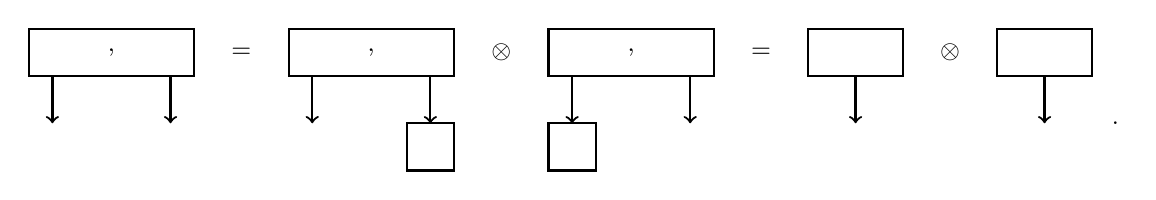
\begin{tikzpicture}[scale=0.3,thick] % , baseline = -3.5pt


\draw (0,1) rectangle (7,-1);
\node[anchor=center] (text) at (3.5,0) {\small $\probat{\exrandom,\secexrandom}$};
\draw[->] (1,-1) -- (1,-3) node[midway, left] {\tiny $\exrandom$};
\draw[->] (6,-1) -- (6,-3) node[midway, left] {\tiny $\secexrandom$};

\node[anchor=center] (text) at (9,0) {\small ${=}$};


\begin{scope}[shift={(11,0)}]

\draw (0,1) rectangle (7,-1);
\node[anchor=center] (text) at (3.5,0) {\small $\probat{\exrandom,\secexrandom}$};
\draw[->] (1,-1) -- (1,-3) node[midway, left] {\tiny $\exrandom$};
\draw[->] (6,-1) -- (6,-3) node[midway, left] {\tiny $\secexrandom$};
\draw (5,-3) rectangle (7,-5);
\node[anchor=center] (text) at (6,-4) {\small $\ones$};

\end{scope}

\node[anchor=center] (text) at (20,0) {\small $\otimes$};

\begin{scope}[shift={(22,0)}]

\draw (0,1) rectangle (7,-1);
\node[anchor=center] (text) at (3.5,0) {\small $\probat{\exrandom,\secexrandom}$};
\draw[->] (1,-1) -- (1,-3) node[midway, left] {\tiny $\exrandom$};
\draw (0,-3) rectangle (2,-5);
\node[anchor=center] (text) at (1,-4) {\small $\ones$};
\draw[->] (6,-1) -- (6,-3) node[midway, left] {\tiny $\secexrandom$};

\end{scope}

\node[anchor=center] (text) at (31,0) {\small ${=}$};

\begin{scope}[shift={(33,0)}]

\draw (0,1) rectangle (4,-1);
\node[anchor=center] (text) at (2,0) {\small $\margprobat{\exrandom}$};
\draw[->] (2,-1) -- (2,-3) node[midway, left] {\tiny $\exrandom$};

\node[anchor=center] (text) at (6,0) {\small $\otimes$};

\draw (8,1) rectangle (12,-1);
\node[anchor=center] (text) at (10,0) {\small $\margprobat{\secexrandom}$};
\draw[->] (10,-1) -- (10,-3) node[midway, left] {\tiny $\secexrandom$};


\end{scope}

\node[anchor=center] (text) at (46,-3) {\small ${.}$};

\end{tikzpicture} 
\end{center}
Let us notice, that the assumption of independence reduces the degrees of freedom from $\exranddim\cdot\secexranddim-1$ to $(\exranddim-1)+(\secexranddim-1)$.
The decomposition by marginal distributions furthermore exploits this reduced freedom and provides an efficient storage.
Having a joint distribution of multiple variables, which disjoint subsets are independent, we can iteratively apply the decomposition scheme.
As a result, the degrees of freedom scaling exponential in the number of distributed variables would be reduced to a linear scaling, by the assumption of independence.

% Motivation of conditional independence as more realistic property
Independence is, as we observed, a strong assumption, which is often too restrictive.
It is furthermore an undesired property, when in a supervised learning scenario a target variable has to be predicted based on known feature variables.
Conditional independence instead is a less demanding assumption, which still implies efficient tensor network decompositions schemes.
We introduce conditional independence as independence of variables with respect to conditional distributions.

\begin{definition}[Conditional Independence]
    \label{def:condIndependence}
    Given a joint distribution of variables $\exrandom$, $\secexrandom$ and $\thirdexrandom$, such that $\margprobat{\thirdexrandom}$ is positive.
    We say that $\exrandom$ is independent of $\secexrandom$ conditioned on $\thirdexrandom$ if for any states $\exrandindin,\secexrandindin$ and $\thirdexrandindin$
    \begin{align*}
        \condprobof{\indexedexrandom,\indexedsecexrandom}{\indexedthirdexrandom}
        = \condprobof{\indexedexrandom}{\indexedthirdexrandom}
        \cdot \condprobof{\indexedsecexrandom}{\indexedthirdexrandom}   \, .
    \end{align*}
    In this case we denote $\condindependent{\exrandom}{\secexrandom}{\thirdexrandom}$.
\end{definition}

Conditional independence stated in \defref{def:condIndependence} has a close connection with independence stated in \defref{def:independence}.
To be more precise, $\exrandom$ is independent of $\secexrandom$ conditioned on $\thirdexrandom$, if and only if $\exrandom$ is independent of $\secexrandom$ with respect to any slice $\condprobof{\exrandom,\secexrandom}{\thirdexrandom=\thirdexrandind}$ of the conditional distribution $\condprobof{\exrandom,\secexrandom}{\thirdexrandom}$.
Analogously to \theref{the:independenceProductCriterion} for independence, we further find a decomposition criterion for conditional independence.
Since conditional independence can be regarded as a property of conditional probabilities, this decomposition criterion also involves conditional probabilities.

\begin{theorem}[Conditional Independence as a Contraction Equation]
    \label{the:condIndependenceProductCriterion}
    Given a distribution $\probtensor$ of variables $\exrandom$, $\secexrandom$ and $\thirdexrandom$, the variable $\exrandom$ is independent of $\secexrandom$ conditioned on $\thirdexrandom$, if and only if the equation
    \begin{align*}
        \condprobof{\exrandom,\secexrandom}{\thirdexrandom}
        = \contractionof{
            \condprobof{\exrandom}{\thirdexrandom},\condprobof{\secexrandom}{\thirdexrandom}
        }{\exrandom,\secexrandom,\thirdexrandom}
    \end{align*}
    holds.
\end{theorem}
\begin{proof}
    With the same argumentation as in the proof of \theref{the:independenceProductCriterion}, we notice that the contraction equation holds, if and only if for any $\exrandindin$, $\secexrandindin$ and $\thirdexrandindin$
    \begin{align*}
        \condprobof{\indexedexrandom,\indexedsecexrandom}{\indexedthirdexrandom}
        = \condprobof{\indexedexrandom}{\indexedthirdexrandom} \cdot \condprobof{\indexedsecexrandom}{\indexedthirdexrandom} \, .
    \end{align*}
    This is equivalent to conditional independence by \defref{def:condIndependence}.
\end{proof}

We can further exploit conditional independence to find tensor network decompositions of probabilities, as we show as the next corollary.
\begin{figure}[hbt!]
    \begin{center}
        \begin{tikzpicture}[scale=0.3,thick] % , baseline = -3.5pt


\draw (-2,1) rectangle (7,-1);
\node[anchor=center] (text) at (2.5,0) {\corelabelsize $\probat{\exrandom,\secexrandom,\thirdexrandom}$};
\draw[->-] (-1,-1) -- (-1,-3) node[midway, left] {\colorlabelsize $\exrandom$};
\draw[->-] (2.5,-1) -- (2.5,-3) node[midway, left] {\colorlabelsize $\secexrandom$};
\draw[->-] (6,-1) -- (6,-3) node[midway, left] {\colorlabelsize $\thirdexrandom$};

\node[anchor=center] (text) at (9,0) {\corelabelsize ${=}$};

\draw (11,1) rectangle (18,-1);
\node[anchor=center] (text) at (14.5,0) {\corelabelsize $\condprobof{\exrandom}{\thirdexrandom}$};
\draw[->-] (12,-1) -- (12,-3) node[midway, left] {\colorlabelsize $\exrandom$};
\draw[-<-] (17,-1) -- (17,-3) node[midway, left] {\colorlabelsize $\thirdexrandom$};

\draw (21,1) rectangle (25,-1);
\node[anchor=center] (text) at (23,0) {\corelabelsize $\probat{\thirdexrandom}$};
\draw (23,-1) -- (23,-3) node[midway, left] {\colorlabelsize $\thirdexrandom$};

\draw (23,-3) -- (23,-5);
\draw[fill] (23,-5) circle (\dotsize);
\draw[->-] (23,-5) -- (23,-7) node[midway, left] {\colorlabelsize $\thirdexrandom$};
\draw (17,-3) to[bend right=40] (23,-5);
\draw (29,-3) to[bend right=-40] (23,-5);


\draw (28,1) rectangle (35,-1);
\node[anchor=center] (text) at (31.5,0) {\corelabelsize $\condprobof{\secexrandom}{\thirdexrandom}$};
\draw[-<-] (29,-1) -- (29,-3) node[midway, left] {\colorlabelsize $\thirdexrandom$};
\draw[->-] (34,-1) -- (34,-3) node[midway, left] {\colorlabelsize $\secexrandom$};



\end{tikzpicture} 
    \end{center}
    \caption{Diagrammatic visualization of the contraction equation in \corref{cor:secCriterionCondIndepencence}.
    Conditional independence of $\exrandom$ and $\secexrandom$ given $\thirdexrandom$ holds if the contraction on the right ride is equal to the probability tensor on the left side.}
    \label{fig:condIndependenceDecomposition}
\end{figure}


\begin{corollary}
    \label{cor:secCriterionCondIndepencence}
    %Let $\probat{\exrandom,\secexrandom,\thirdexrandom}$ be a distribution, such that
    If and only if $\exrandom$ is independent of $\secexrandom$ conditioned on $\thirdexrandom$ the probability distribution $\probtensor$ satisfies (see \figref{fig:condIndependenceDecomposition})
    \begin{align*}
        \probat{\exrandom,\secexrandom,\thirdexrandom}
        = \contractionof{\condprobof{\exrandom}{\thirdexrandom},\condprobof{\secexrandom}{\thirdexrandom},\margprobat{\thirdexrandom}}{\exrandom,\secexrandom,\thirdexrandom} \, .
    \end{align*}
\end{corollary}
\begin{proof}
    With the Bayes \theref{the:bayes} it holds that
    \begin{align*}
        \probat{\exrandom,\secexrandom,\thirdexrandom}
        = \contractionof{\condprobof{\exrandom,\secexrandom}{\thirdexrandom},\margprobat{\thirdexrandom}}{\exrandom,\secexrandom,\thirdexrandom} \, .
    \end{align*}
    Decomposing the first tensor in the contraction, \theref{the:condIndependenceProductCriterion} implies, that $\exrandom$ is independent of $\secexrandom$ conditioned on $\thirdexrandom$, if and only if
    \begin{align*}
        \probat{\exrandom,\secexrandom,\thirdexrandom}
        = \contractionof{\condprobof{\exrandom}{\thirdexrandom},\condprobof{\secexrandom}{\thirdexrandom},\margprobat{\thirdexrandom}}{\exrandom,\secexrandom,\thirdexrandom} \, .
    \end{align*}
\end{proof}


Let us now recall our motivation of the study of conditional independence, namely to find sparsifications of conditional probabilities as those appearing in chain decompositions \theref{the:chainRule}.
As we state as the next theorem, such sparsifications follow from conditional independence.
%Conditional independence can be exploited in the sparsification of conditional probabilities.

\begin{theorem}
    \label{the:conditionDropping}
    Whenever $\exrandom$ is independent of $\secexrandom$ given $\thirdexrandom$, we have for any $\secexrandindin$
    \begin{align*}
        \condprobof{\exrandom}{\indexedsecexrandom,\thirdexrandom}
        = \condprobof{\exrandom}{\thirdexrandom} \, .
    \end{align*}
\end{theorem}
\begin{proof}
    By the Bayes \theref{the:bayes} we have for any indices to the variables
    \begin{align*}
        \condprobof{\indexedexrandom}{\indexedsecexrandom,\indexedthirdexrandom}
        = \frac{\condprobof{\indexedexrandom,\indexedsecexrandom}{\indexedthirdexrandom}}{
            \contraction{\condprobof{\exrandom,\indexedsecexrandom}{\indexedthirdexrandom}}
        }
    \end{align*}
    If $\exrandom$ is independent of $\secexrandom$ given $\thirdexrandom$ it follows that
    \begin{align*}
        \condprobof{\indexedexrandom}{\indexedsecexrandom,\indexedthirdexrandom}
        & = \frac{\condprobof{\indexedexrandom}{\indexedthirdexrandom} \cdot \condprobof{\indexedsecexrandom}{\indexedthirdexrandom}}{
            \contraction{\condprobof{\exrandom,\indexedsecexrandom}{\indexedthirdexrandom}}
        } \\
        & = \condprobof{\indexedexrandom}{\indexedthirdexrandom} \, .
    \end{align*}
\end{proof}

Following our motivation of sparse decompositions, we now combine this result with the generic chain rule, to show Markov Chain decompositions.
\begin{figure}[h]
    \begin{center}
        \begin{tikzpicture}[scale=0.3,thick] % , baseline = -3.5pt

\node[anchor=center] (text) at (-1,3) {${a)}$};

	\node [circle, draw, thick, fill=gray!50] (T1) at (0,0) {\tiny $\randomxof{0}$};
	\node [circle, draw, thick, fill=gray!50] (T2) at (5,0) {\tiny $\randomxof{1}$};
	\draw[->-] (T1) -- (T2);
	\node [circle, draw, thick, fill=gray!50] (T3) at (10,0) {\tiny $\randomxof{2}$};
	\draw[->-] (T2) -- (T3);
	\node [circle, draw, thick, fill=gray!50] (T4) at (15,0) {\tiny $\randomxof{3}$};
	\draw[->-] (T3) -- (T4);
	\draw[->-] (T4) -- (18,0);

	\node[anchor=center] (text) at (19,0) {$\cdots$};

	%\node [circle, draw, thick, fill=gray!50] (T4) at (17,0) {\tiny $\randomxof{\atomorder}$};
	%\draw[->-] (14,0) -- (T4);
			

\begin{scope}[shift={(25,0)}]

\node[anchor=center] (text) at (-3,3) {${b)}$};

\draw (-3.5,-1) rectangle (0, 1);
\node[anchor=center] (text) at (-1.75,0) {\small $\probat{\randomxof{0}}$};
\draw[->-] (0,0) -- (2,0);
\draw[fill] (1,0) circle (0.15cm);
\draw[->-] (1,0) -- (1,2) node[above] {\tiny $\catvariableof{0}$};
\draw (2,-1) rectangle (7, 1);
\node[anchor=center] (text) at (4.5,0) {\small $\condprobof{\randomxof{1}}{\randomxof{0}}$};
\draw[->-]  (7,0) -- (9,0);
\draw[fill] (8,0) circle (0.15cm);
\draw[->-] (8,0) -- (8,2) node[above] {\tiny $\catvariableof{1}$};
\draw (9,-1) rectangle (14, 1);
\node[anchor=center] (text) at (11.5,0) {\small $\condprobof{\randomxof{2}}{\randomxof{1}}$};
\draw[->-]  (14,0) -- (16,0);
\draw[fill] (15,0) circle (0.15cm);
\draw[->-] (15,0) -- (15,2) node[above] {\tiny $\catvariableof{2}$};
\draw (16,-1) rectangle (21, 1);
\node[anchor=center] (text) at (18.5,0) {\small $\condprobof{\randomxof{3}}{\randomxof{2}}$};
\draw[->-]  (21,0) -- (23,0);
\draw[fill] (22,0) circle (0.15cm);
\draw[->-] (22,0) -- (22,2) node[above] {\tiny $\catvariableof{3}$};
\node[anchor=center] (text) at (24,0) {$\cdots$};


\end{scope}

\end{tikzpicture} 
    \end{center}
    \caption{Depiction of a Markov Chain Decomposition by a
    a) hypergraph with the nodes $\nodes=[\catorder]$ and edges $\edges=\big\{\{0\}\cup\{\{\catenumerator,\catenumerator+1\} \, : \, \catenumeratorin, \, \catenumerator>1\} \big\}$ and
    b) a decorating Tensor Network representing the sparsified conditional probabilities.}
    \label{fig:MC}
\end{figure}

% More of an example?
\begin{theorem}[Markov Chain]
    \label{the:MarkovChain}
    Let there be a set of variables $\catvariableof{\catenumerator}$ where $\catenumeratorin$, and let us denote for $\catenumeratorin$ by $\catvariableof{[\catenumerator]}$ the collection of variables $\catvariableof{0},\ldots,\catvariableof{\catenumerator-1}$.
    Let us assume, that for any $\catenumeratorin$ with $\catenumerator\geq2$ the variable $\catvariableof{\catenumerator}$ is independent of $\catvariableof{[\catenumerator-1]}$ conditioned on $\catvariableof{\catenumerator-1}$, then
    \begin{align*}
        \probwith
        = \contractionof{\{\margprobat{\catvariableof{0}}\} \cup \{\condprobof{\catvariableof{\catenumerator}}{\catvariableof{\catenumerator-1}}\,:\,\catenumeratorin, \, \catenumerator\geq1\}}{\shortcatvariables}
    \end{align*}
%    Here we denote by $\condprobof{\catvariableof{0}}{\catvariableof{-1}}$ the marginal distribution of $\margprobat{\catvariableof{0}}$.
    We depict this decomposition in \figref{fig:MC}.
\end{theorem}
\begin{proof}
    By the chain rule shown in \theref{the:chainRule} we have
    \begin{align*}
        \probwith
        = \contractionof{
            \{ \condprobof{\catvariableof{\catenumerator}}{\catvariableof{[\catenumerator]}} \,:\, \catenumeratorin \}
        }{\shortcatvariables}
    \end{align*}
    Using that $\catvariableof{\catenumerator}$ is conditional independent of $\catvariableof{[\catenumerator-1]}$ conditioned on $\catvariableof{\catenumerator-1}$ we further have by \theref{the:conditionDropping}
    \begin{align*}
        \condprobof{\catvariableof{\catenumerator}}{\catvariableof{[\catenumerator]}}
        = \condprobof{\catvariableof{\catenumerator}}{\catvariableof{\catenumerator-1}} \otimes \onesat{\catvariableof{[\catenumerator-1]}} \, .
    \end{align*}
    Composing both equalities and omitting the trivial tensors shows the claim.
\end{proof}

% Markov Property
The assumption of $\catvariableof{\catenumerator}$ being independent of $\catvariableof{[\catenumerator-1]}$ conditioned on $\catvariableof{\catenumerator-1}$ is called the Markov property and the corresponding collection of random variables is called a Markov Chain.
\theref{the:MarkovChain} states an efficient decomposition of the probability distribution into a concatenated product of matrices representing conditional probability distributions.
Marginal distributions of Markov Chains can therefore consecutively be computed by matrix-vector products, that is for $\catenumeratorin$ with $\catenumerator\geq1$
\begin{align*}
    \margprobat{\catvariableof{\catenumerator}}
    = \contractionof{\condprobat{\catvariableof{\catenumerator}}{\catvariableof{\catenumerator-1}},\margprobat{\catvariableof{\catenumerator-1}}}{\catvariableof{\catenumerator}} \, .
\end{align*}
The conditional probability matrices are therefore called stochastic transition matrices.

We notice, that the decomposition scheme of \theref{the:MarkovChain} hints at an efficient representation of $\probwith$ based on transition matrices.
While $\probwith$ is a tensor in a space of dimension
\begin{align*}
    \prod_{\catenumeratorin} \catdimof{\catenumerator} \, ,
\end{align*}
the sum of the dimension of the transition matrices is
\begin{align*}
    \catdimof{0} + \sum_{\catenumeratorin,\, \catenumerator\geq 1} \catdimof{\catenumerator}\cdot \catdimof{\catenumerator-1} \, .
\end{align*}
We therefore observe a linear increase of the storage demand of the transition matrices in the order $\catorder$, whereas a naive storage of $\probwith$ by its coordinates would have an exponentially demand.

% Generalizing Markov Chain
The Markov Chain serves as a toy example drawing on a restrictive chain arrangement of conditional independencies.
In the following section, we will investigate decomposition schemes, which relax this assumption and draw on more general collections of conditional independencies.
The computation of marginal distribution by consecutive transition matrix multiplications will then be replaced by more general tensor network contractions.



\sect{Sufficient Statistics and Exponential Families}\label{sec:exponentialFamilies}

\red{We have seen, that conditional independence of variables corresponds with decomposition properties of probability tensors.
Another mechanism is through sufficient statistics, which leads to exponential families.
When restricting to graphical models in the next section, we will see that both mechanisms are related through the Hammersley-Clifford theorem.}

\subsect{Sufficient Statistics}

Let us consider a tuple of random variables $\shortcatvariables$, which take values in $\facstates$.
We now understand the probability $\probat{\shortcatvariables}$ as another random variable taking values in $[0,1]$, which has a deterministic dependence on $\shortcatvariables$.

\begin{definition}[Sufficient Statistics]
    Let $\shortcatvariables$ be a tuple of by $\probat{\shortcatvariables}$ jointly distributed random variables and $\sstatat{\shortcatvariables,\selvariable}$ be a tensor.
    We consider the tuple of random variables $(\shortcatvariables,\probat{\shortcatvariables},\sstatat{\shortcatvariables,\selvariable})$, which takes for $\shortcatindices\in\facstates$ with probability $\probat{\indexedshortcatvariables}$ the value
    \begin{align*}
        \left(\shortcatindices,\probat{\indexedshortcatvariables},\sstatat{\indexedshortcatvariables,\selvariable}\right) \, .
    \end{align*}
    We say, that $\sstat$ is a sufficient statistic for $\probtensor$, if this tuple obeys
    \begin{align*}
        \condindependent{\shortcatvariables}{\probat{\shortcatvariables}}{\sstatat{\shortcatvariables,\selvariable}} \, .
    \end{align*}
\end{definition}

%In the notation of this reads as
%\begin{align*}
%    \shortcatvariables\rightarrow\probat{\shortcatvariables} \, .
%\end{align*}

%A sufficient statistic is another random variables $\sstatat{\shortcatvariables,\selvariable}$ taking values in $\rr^{\seldim}$, such that $\shortcatvariables$ is independent of $\probat{\shortcatvariables}$ conditioned on $\sstatat{\shortcatvariables,\selvariable}$.
%We then have a Markov Chain (see \cite{cover_elements_2006})
%\begin{align*}
%    \shortcatvariables \rightarrow \sstatat{\shortcatvariables} \rightarrow \probat{\shortcatvariables} \, .
%\end{align*}


\begin{theorem}\label{the:sufficientStatisticActCoreExistence}
    If and only if $\sstatat{\shortcatvariables,\selvariable}$ is a sufficient statistic, i.e. $\shortcatvariables$ is independent of $\probat{\shortcatvariables}$ conditioned on $\sstatat{\shortcatvariables,\selvariable}$, there is a tensor $\actcoreat{\headvariableof{[\seldim]}}$ with
    \begin{align*}
        \probat{\shortcatvariables} = \contractionof{\rencodingofat{\sstat}{\headvariableof{[\seldim]},\shortcatvariables},\actcoreof{\headvariableof{[\seldim]}}}{\shortcatvariables} \, .
    \end{align*}
\end{theorem}
\begin{proof}
    We exploit conditional entropies, for which definition we refer to Chapter~2 in \cite{cover_elements_2006}. % Can we avoid that and directly refer?
    By the data processing inequality (see e.g. Theorem~2.8.1 in \cite{cover_elements_2006}), we have
    \begin{align*}
        \sentropyof{\probtensor|\sstat} \leq \sentropyof{\probtensor |\shortcatvariables} = 0
    \end{align*}
    and thus $\sentropyof{\probtensor|\sstat}=0$.
    Moreover, $\sentropyof{\probtensor|\sstat}=0$ is equivalent to a straight satisfaction of the data processing inequality, and $\sstat$ being a sufficient statistic for $\probtensor$.
    $\sentropyof{\probtensor|\sstat}=0$ is furhter equivalent to the existance of a function $\exfunction:\rr^{\seldim}\rightarrow[0,1]$, such that for each $\shortcatindices$
    \begin{align*}
        \exfunctionof{\sstatat{\indexedshortcatvariables,\selvariable}} = \probat{\indexedshortcatvariables} \, .
    \end{align*}
    For an index interpretation function $\indexinterpretation$, enumerating $\bigtimes_{\selindexin}\imageof{\sstatcoordinateof{\selindex}}$ using the variables $\headvariableof{[\seldim]}$, we define
    \begin{align*}
        \actcore := \exfunction \circ \indexinterpretation \, .
    \end{align*}
    Using basis calculus (see \charef{cha:basisCalculus}) and in particular \theref{the:tensorFunctionComposition} we have
    \begin{align*}
        \probat{\shortcatvariables} = \contractionof{\rencodingofat{\sstat}{\headvariableof{[\seldim]},\shortcatvariables},\actcoreof{\headvariableof{[\seldim]}}}{\shortcatvariables} \, .
    \end{align*}
\end{proof}

Given a statistic $\sstat$, we can thus characterize the set of probability distributions, for which $\sstat$ is sufficient, as
\begin{align*}
    \realizabledistsof{\sstat,\maxgraph}
    := \left\{\normationof{\rencodingofat{\sstat}{\headvariableof{[\seldim]},\shortcatvariables},\actcoreof{\headvariableof{[\seldim]}}}{\shortcatvariables} \right\}
\end{align*}
%where by $\maxgraph$ we refer to the maximal graph to be explained later


% Usage of the selection encoding -> Can also make a theorem out of this

\subsect{Exponential families}

\red{\theref{the:sufficientStatisticActCoreExistence} states the existance of an activation core, once a sufficient vector statistic has been identified.
However, since the dimension of the activation core space is increasing exponential with the number of features (it is the product of the image cardinalities of the features), representation of generic $\actcore$ is not feasible.
We now restrict the activation cores to specific elementary tensors, which correspond with further assumptions on the dependence of $\probtensor$ and $\sstat$ made by exponential families.}

The probability distributions, which are members of an exponential family, share the computation of the probability tensor based on a boolean base measure, marking the support of the distribution, and a statistic function containing features.
They differ only by canonical parameters which weight the features at a given state to calculate the respective probability.
Exponential families consist the most generic distributions investigated in this work and will also serve as a generic framework in the discussion of probabilistic reasoning in \charef{cha:probReasoning}, as well as for neuro-symbolic models in \parref{par:two}.

%where each coordinate is determined by a base measure and a set $\sstat$ of features as
%\[ \probat{\indexedshortcatvariables}  \propto \basemeasure(\catindex) \cdot \expof{\sum_{\selindexin} \sstatcoordinateofat{\selindex}{\indexedshortcatvariables} \cdot \canparamat{\indexedselvariable}} \, . \]


\begin{definition}
    \label{def:expFamily}
    Given a statistic function
    \begin{align*}
        \sstat : \facstates \rightarrow \parspace
    \end{align*}
    and a boolean base measure
    \begin{align*}
        \basemeasure : \facstates \rightarrow \ozset
    \end{align*}
    with $\contraction{\basemeasure}\neq0$, the set $\expfamily=\{\expdist \, : \, \canparamwithin\}$ of probability distributions
    \begin{align*}
        \expdistat{\shortcatvariables} = \normationof{\expof{\sbcontractionof{\sencsstatat{\shortcatvariables,\selvariable},\canparamwith}{\shortcatvariables},\basemeasurewith}}{\shortcatvariables}
    \end{align*}
    is called the exponential family to $\sstat$.
    We further define for each member with parameters $\canparam$ the associated energy tensor
    \begin{align*}
        \expenergy = \sbcontractionof{\sencsstat,\canparam}{\shortcatvariables}
    \end{align*}
    and the cumulant function
    \[ \cumfunctionof{\canparam} = \lnof{\sbcontraction{\basemeasure,\expof{\sbcontractionof{\sencsstat,\canparam}{\shortcatvariables} }} } \, .\]
\end{definition}


We used the selection encoding to represent the weighted summation over the statistics, that is the tensor (see \defref{def:selectionEncoding})
\begin{align*}
    \sencsstatat{\shortcatvariables,\selvariable}: \facstates \times [\seldim] \rightarrow \rr
\end{align*}
defined for $\shortcatindices\in\facstates$ and $\selindexin$ as
\begin{align*}
    \sencsstatat{\indexedshortcatvariables,\indexedselvariable} = \sstatcoordinateofat{\selindex}{\indexedshortcatvariables} \, .
\end{align*}
The selection encoding represent the weighted sum of the statistic coordinates by the canonical parameter vector $\canparamwith$ as a contraction
\begin{align*}
    \sum_{\selindexin}\canparamat{\indexedselvariable}\cdot \sstatcoordinateofat{\selindex}{\shortcatvariables}
    = \sbcontractionof{\sencsstatat{\shortcatvariables,\selvariable},\canparamwith}{\shortcatvariables} \, .
\end{align*}
For more details on this representation scheme, we refer to \theref{the:linCompSelEncoding} in \charef{cha:coordinateCalculus}.
Up to normation, we sketch the probability distribution of any member by the tensor network diagram
\begin{center}
    \begin{tikzpicture}[scale=0.35,thick] % , baseline = -3.5pt

    \begin{scope}
        [shift={(-20,-8)}]

        \draw (-6,1) rectangle (10, 4);
        \node[anchor=center] (text) at (2,2.5) {\small $\contractionof{\expof{\sbcontractionof{\sencsstat,\canparam}{\shortcatvariables},\basemeasureat{\shortcatvariables}}}{\shortcatvariables}$};

        \draw[] (0,1)--(0,-1) node[midway,left] {\tiny $\catvariableof{0}$};
        \draw[] (0,-1)--(0,-1.5);
        \draw[] (1.5,1)--(1.5,-1) node[midway,left] {\tiny $\catvariableof{1}$};
        \draw[] (1.5,-1)--(1.5,-1.5);
        \node[anchor=center] (text) at (3,0) {$\cdots$};
        \draw[] (4,1)--(4,-1) node[midway,right] {\tiny $\catvariableof{\atomorder\shortminus1}$};
        \draw[] (4,-1)--(4,-1.5);

        \node[anchor=center] (text) at (12,1.5) {${=}$};
    \end{scope}

    \begin{scope}
        [shift={(0,-4)}]
        \draw[] (0,1)--(0,-6);
        \node[below] (text) at (0,-6) {\tiny $\catvariableof{\atomorder\shortminus1}$};
        \drawvariabledot{0}{-5}
        \draw[] (1.5,1)--(1.5,-6);
        \node[below] (text) at (1.5,-6) {\tiny $\catvariableof{1}$};
        \drawvariabledot{1.5}{-3}
        \node[anchor=center] (text) at (3,0) {$\cdots$};
        \node[anchor=center] (text) at (3,-5.5) {$\cdots$};
        \draw[] (4,1)--(4,-6);
        \node[below] (text) at (4,-6) {\tiny $\catvariableof{\atomorder\shortminus1}$};
        \drawvariabledot{4}{-2}

        \draw[] (0,-5) -- (6,-5);
        \draw[] (1.5,-3) -- (6,-3);
        \node[anchor=center] (text) at (5,-3.75) {$\vdots$};
        \draw[] (4,-2) -- (6,-2);
        \draw (6,-1) rectangle (9, -6);
        \node[anchor=center] (text) at (7.5,-3.5) {$\basemeasure$};

        \node[anchor=center] (text) at (10,-4.5) {$.$};

    \end{scope}

    \draw (-1,-3) rectangle (5, 0);
    \node[anchor=center] (text) at (2,-1.5) {$\sencsstat$};

    \draw[] (5,-2)--(7,-2) node[midway,below] {\tiny $\selvariable$};
    \draw (7,-3) rectangle (9, -1);
    \node[anchor=center] (text) at (8,-2) {$\canparam$};

    \node[anchor=center] (text) at (-3.5,-2) {\small $\mathrm{exp}$};
    \draw (2,-2) ellipse (8 and 2.75);

\end{tikzpicture}
\end{center}
We here denote by an ellipsis the coordinatewise transformation by the exponential function (see \secref{sec:coordinatewiseTransforms}).
Since such coordinatewise transformation are nonlinear, they are a caveat for efficient contraction of the diagram.

% Diverging partition functions avoided here
Since we restrict the discussion to finite state spaces, the distribution $\expdist$ is well-defined for any $\canparamwith\in\parspace$.
For infinite state space there are sufficient statistics and parameters, such that the partition function $\sbcontraction{\basemeasure,\expof{\sbcontractionof{\sencsstat,\canparam}{\shortcatvariables}}}$ diverges and the normation $\expdist$ is not well-defined.
In that cases, the canonical parameters need to be chosen from a subset where the partition function is finite \cite{wainwright_graphical_2008}.

% Restriction to boolean base measures
As before, we restrict to boolean base measures, which have to satisfy $\contraction{\basemeasure}\neq0$ for respective distributions to exist.
We notice, that by positivity of the exponential function, any distribution in an exponential family $\expfamily$ is positive with respect to $\basemeasure$ (see \defref{def:positivityBaseMeasure}).
In \charef{cha:networkRepresentation} we will investigate distributions, where the base measures and the sufficient statistics share a common decomposition framework.

% Cumulant representation
\begin{lemma}
    \label{lem:energyCumulantRepresentation}
    For any member of an exponential family $\expfamily$ we have
    \begin{align*}
        \expdistat{\shortcatvariables}
        = \contractionof{\expof{ \expenergy - \cumfunctionof{\canparam}\cdot \onesat{\shortcatvariables}},\basemeasureof{\shortcatvariables}}{\shortcatvariables} \, .
    \end{align*}
\end{lemma}
\begin{proof}
    By definition we have
    \begin{align*}
        \expdistat{\shortcatvariables}
        &= \normationof{
            \expof{\sbcontractionof{\sencsstat,\canparam}{\shortcatvariables}},\basemeasurewith
        }{\shortcatvariables} \\
        &= \frac{\contractionof{\expof{\sbcontractionof{\sencsstat,\canparam}{\shortcatvariables},\basemeasurewith}}{\shortcatvariables}
        }{\contraction{\expof{\sbcontractionof{\sencsstat,\canparam    }{\shortcatvariables}},\basemeasurewith}} \\
        &=  \frac{
            \contractionof{\expof{\expenergyat{\shortcatvariables}},\basemeasurewith}{\shortcatvariables}
        }{
            \expof{\cumfunctionof{\canparam}}
        } \\
        & = \contractionof{\expof{ \expenergy - \cumfunctionof{\canparam}\cdot \onesat{\shortcatvariables}},\basemeasureof{\shortcatvariables}}{\shortcatvariables} \, .
    \end{align*}
\end{proof}


% Minimal statistics
A further useful criterion is that of minimality of an exponential family, as we define next.

\begin{definition}[Minimal]
    \label{def:minimalStatistics}
    We say that a statistic $\sstat$ is minimal with respect to a boolean base measure $\basemeasure$, if there is no pair of a non-vanishing vector $\vectorat{\selvariable}$ and a scalar $\lambda\in\rr$ with
    \begin{align*}
        \contractionof{\sencsstatat{\shortcatvariables,\selvariable},\vectorat{\selvariable},\basemeasurewith}{\shortcatvariables} = \lambda\cdot\basemeasurewith \, .
    \end{align*}
\end{definition}

% Making a statistic minimal
If a statistic is not minimal, we can omit coordinates of it without affecting the expressivity $\expfamily$.
As long as we find a non-vanishing vector $\vectorat{\selvariable}$ and $\lambda\in\rr$ as in \defref{def:minimalStatistics}, we can choose a coordinate $\sstatcoordinateof{\selindex}$ such that $\vectorat{\indexedselvariable}\neq0$, conclude that the coordinate is linear dependent on the others and drop it as redundant.


\subsect{Tensor Network Representation}

As we have observed, the selection encoding formalism can efficiently represent the energy tensor to a member of an exponential family, but through coordinatewise transform by the exponential does not provide an efficient decomposition scheme of the probability distribution itself.
We now overcome this problem with usage of the relational encoding formalism to represent members of exponential families by a single contraction without nonlinear transforms.
%The central insight here is a relational encoding of the statistic , which enables representation by tensor network decomposition, when the sufficient statistic is decomposable.

\begin{theorem}[Generic Representation of Exponential Families]
    \label{the:expFamilyTensorRep}
    Given any base measure $\basemeasure$ and a sufficient statistic $\sstat$ we enumerate for each coordinate $\selindexin$ the image $\imageof{\sstatcoordinateof{\selindex}}$ by a variable $\sstatcatof{\selindex}$ taking values in $[\cardof{\imageof{\sstatcoordinateof{\selindex}}}]$ (see for more details on this scheme \charef{cha:basisCalculus}), given an interpretation map
    \begin{align*}
        \indexinterpretationof{\selindex} :
        [\cardof{\imageof{\sstatcoordinateof{\selindex}}}] \rightarrow \imageof{\sstatcoordinateof{\selindex}} \, .
    \end{align*}
    For any canonical parameter vector $\canparamwithin$ we build the activation cores
    \begin{align*}
        \actcoreofat{\selindex,\canparamat{\indexedselvariable}}{\indexedheadvariableof{\selindex}}
        = \expof{\canparamat{\indexedselvariable} \cdot \indexinterpretationofat{\selindex}{\headindex{\selindex}} } \,
    \end{align*}
    and have
    \begin{align*}
        \expdistwith =
        \normationof{\{\basemeasurewith\} \cup \{\rencodingofat{\sstatcoordinateof{\selindex}}{\sstatcatof{\selindex},\shortcatvariables} \, : \, \selindexin\}\cup\{\sstatac \, : \, \selindexin\}}{\shortcatvariables} \, .
    \end{align*}
\end{theorem}
\begin{proof}
    We embed the image of $\sstat$ in the cartesian product of the coordinate images  %	which does not modify the statement of Theorem~\ref{the:tensorFunctionComposition} (since extension to cases, which are never met).
    \begin{align*}
        \imageof{\sstat} \subset \bigtimes_{\selindexin} \imageof{\sstatcoordinateof{\selindex}} \,
    \end{align*}
    and design enumerate the embedded image of $\sstat$ by the variables $\sstatcatof{[\seldim]}$.
    \theref{the:tensorFunctionComposition}, to be shown in \charef{cha:basisCalculus}, implies
    \begin{align*}
        \expof{\sbcontractionof{\sencsstat,\canparam}{\shortcatvariables}}
        = \contractionof{
            \rencodingofat{\sstat}{\sstatcatof{[\seldim]},\shortcatvariables},\restrictionofto{\expof{\braket{\cdot,\canparamwith}}
            }{\bigtimes_{\selindexin}\imageof{\sstatcoordinateof{\selindex}}}}{\shortcatvariables} \, .
    \end{align*}
    Here we denote by $\braket{\cdot,\canparamwith}$ the dual function to $\canparamwith$, which assigns to vectors their contraction with $\canparamwith$.
    Its restriction onto the vectors in $\bigtimes_{\selindexin}\imageof{\sstatcoordinateof{\selindex}}$ is the tensor satisfying
    \begin{align*}
        \restrictionoftoat{\expof{\braket{\cdot,\canparam}}}{\imageof{\sstat}}{\sstatcatof{[\seldim]}}
        = \bigotimes_{\selindexin} \restrictionoftoat{\expof{\cdot \canparamat{\indexedselvariable}}}{\imageof{\sstatcoordinateof{\selindex}}}{\sstatcatof{\selindex}}
        = \bigotimes_{\selindexin} \actcoreofat{\selindex,\canparamat{\indexedselvariable}}{\sstatcatof{\selindex}} \, .
    \end{align*}
    We further have (see \theref{the:functionImageDecompositionContraction} in \charef{cha:basisCalculus})
    \begin{align*}
        \rencodingofat{\sstat}{\sstatcatof{[\seldim]},\shortcatvariables}
        = \contractionof{\{\rencodingofat{\sstatcoordinateof{\selindex}}{\sstatcatof{\selindex},\shortcatvariables} \, : \, \selindexin\}}{\sstatcatof{[\seldim]},\shortcatvariables} \, .
    \end{align*}
    Refining the above decomposition of $\expof{\sbcontractionof{\sencsstat,\canparam}{\shortcatvariables}}$ by these further decompositions we arrive at the claim.
\end{proof}


In the proof of \theref{the:expFamilyTensorRep} we have observed, that the relational encoding $\rencodingofat{\sstat}{\sstatcatof{[\seldim]},\shortcatvariables}$ of the statistics decomposed into a tensor network of relational encodings $\rencodingofat{\sstatcoordinateof{\selindex}}{\sstatcatof{\selindex},\shortcatvariables}$ to the coordinate of the statistic.
We can exploit further decomposition mechanisms, which will be discussed in full detail in \charef{cha:basisCalculus}, to find even sparser decompositions.
This is for example the case, when the coordinates of the statistic are compositions of functions depending on small numbers of variables.
When the coorindates of the statistic furthermore share similar parts in their compositions, these parts can be shared in the decomposition.
We will investigate such sparsification mechanisms in more detail in \charef{cha:networkRepresentation}, where the coordinates of the statistic are propositional formulas with a natural decomposition by their syntactical description.
%We used in the proof, that the relational encoding of the statistic decomposes into the relational encoding of the coordinate maps to the statistic as
%\begin{align*}
%    \rencodingofat{\sstat}{\sstatcatof{[\seldim]},\shortcatvariables}
%     = \contractionof{\{\rencodingofat{\sstatcoordinateof{\selindex}}{\sstatcatof{\selindex},\shortcatvariables} \, : \, \selindexin\}}{\sstatcatof{[\seldim]},\shortcatvariables} \, .
%\end{align*}
%One strategy to decompose $\rencodingof{\sstat}$ is thus by the .
%When the coordinate maps are sharing common components, a sparser representation can be derived through encodings of the components shared among the coordinate map encodings.


% Core types
The tensor network representation of an exponential family by \theref{the:expFamilyTensorRep} is a Markov Network consistent of two types of cores.
First, we refer to the relational encodings $\rencodingof{\sstatcoordinateof{\selindex}}$ of the coordinates of a statistic as computation cores.
Our intuition is that they compute the hidden variable $\sstatcatof{\selindex}$, based on Basis Calculus (see \charef{cha:basisCalculus}), which encode the value of the coordinate with respect to the image interpretation map $\indexinterpretationof{\selindex}$.
We notice, that since they are directed with $\sstatcatof{\selindex}$ being the only outgoing variable, they do not influence any contraction with open variables $\shortcatvariables$, unless further tensors sharing the variable $\sstatcatof{\selindex}$ are present in the contraction.
The influence of the contraction is performed by the activation cores $\actcoreofat{\selindex,\canparamat{\indexedselvariable}}{\sstatcatof{\selindex}}$, which exploit the computed statistic variable and provide in combination with the relational encoding a factor
\begin{align*}
    \contractionof{\rencodingofat{\sstatcoordinateof{\selindex}}{\sstatcatof{\selindex},\shortcatvariables},\actcoreofat{\selindex,\canparamat{\indexedselvariable}}{\sstatcatof{\selindex}}}{\shortcatvariables}
\end{align*}
to the Markov Network reduced to the observed variables $\shortcatvariables$.
When the canonical parameter is vanishing at a coordinate, that is $\canparamat{\indexedselvariable}=0$, then this factor is trivial, since $\actcoreofat{\selindex,0}{\sstatcatof{\selindex}}=\onesat{\sstatcatof{\selindex}}$ and as a consequence of the directionality of relational encodings we have
\begin{align*}
    \contractionof{\rencodingofat{\sstatcoordinateof{\selindex}}{\sstatcatof{\selindex},\shortcatvariables},\actcoreofat{\selindex,\canparamat{\indexedselvariable}}{\sstatcatof{\selindex}}}{\shortcatvariables}
    = \contractionof{\rencodingofat{\sstatcoordinateof{\selindex}}{\sstatcatof{\selindex},\shortcatvariables},\onesat{\sstatcatof{\selindex}}}{\shortcatvariables}
    = \onesat{\shortcatvariables} \, .
\end{align*}
In that case both the activation core and the corresponding computation core can be dropped from the network without changing its distribution.

% Interpretation as elementary
By \theref{the:expFamilyTensorRep} any member of an exponential family is represented by the normed contraction of a collection of unary activation cores contracted with the computation network $\rencodingofat{\sstat}{\headvariableof{[\seldim]},\shortcatvariables}$.
We understand these activation cores as a member of a simple Markov Network distributing the head variables $\headvariableof{[\seldim]}$.
This Markov Network has a graph, where the edges contain single variables, that is $\elgraph=([\seldim],\{\{\selindex\} \, : \, \selindexin\})$.
We call this graph the elementary graph, since it also corresponds with elementary tensor network formats consistent of tensor products of vectors.
A straightforward generalization of probability distributions representable by exponential families then allows for arbitrary decomposition formats for activation tensors, as we define next.

% Define sets of realizable distributions
\begin{definition}
    \label{def:realizableStatDistributions}
    Given a statistic $\sstat : \facstates \rightarrow \rr^{\seldim}$, and a hypergraph $\graph=([\seldim],\edges)$ with nodes associated to the coordinates of the statistic, we define the by $\sstat$ and $\graph$ computable family of distributions by
    \begin{align*}
        \realizabledistsof{\sstat,\graph}
        = \left\{ \normationof{\{\rencodingofat{\sstat}{\sstatcatof{[\seldim]},\shortcatvariables}\} \cup \{\hypercoreofat{\edge}{\sstatcatof{\edge}}\}}{\shortcatvariables}  \, : \,\hypercoreofat{\edge}{\sstatcatof{\edge}}\in\bigotimes_{\selindex\in\edge}\rr^{\headdimof{\selindex}}, \, \zerosat{\sstatcatof{\edge}}\prec\hypercoreofat{\edge}{\sstatcatof{\edge}} \right\} \, .
    \end{align*}
    Note that we restrict to non-negative activation cores by demanding $\zerosat{\sstatcatof{\edge}}\prec\hypercoreofat{\edge}{\sstatcatof{\edge}}$, a notation which will be introduced in more detail in \charef{cha:logicalReasoning} as partial order of tensors.
    We refer to any member $\probat{\shortcatvariables}\in\realizabledistsof{\sstat,\graph}$ as a by $\sstat$ and $\graph$ computable distribution.
\end{definition}

For unary activation cores, that is for the elementary graph $\elgraph$, any member of $\realizabledistsof{\sstat,\elgraph}$ has up to a normation factor a tensor network decomposition by the diagram
\begin{center}
    \begin{tikzpicture}[scale=0.35,thick,xscale=1] % , baseline = -3.5pt

    \draw (-1.25,1) rectangle (1.25,3);
    \node[anchor=center] (text) at (0,2) {$\actcoreof{{0}}$};

    \draw (2.75,1) rectangle (5.25,3);
    \node[anchor=center] (text) at (4,2) {$\actcoreof{{\seccatorder\shortminus1}}$};

    \draw[->-] (0,-1)--(0,0);
    \node[left] (text) at (0,0) {\tiny $\headvariableof{0}$};
    \draw[] (0,0)--(0,1);
    \drawvariabledot{0}{0}
    \node[anchor=center] (text) at (2,0) {$\cdots$};

    \draw[->-] (4,-1)--(4,0);
    \node[right] (text) at (4,0) {\tiny $\headvariableof{\seccatorder\shortminus1}$};
    \draw[] (4,0)--(4,1);
    \drawvariabledot{4}{0}

    \draw (-1,-1) rectangle (5,-3);
    \node[anchor=center] (text) at (2,-2) {\small $\bencodingof{\sstat}$};
    \draw[-<-] (0,-3)--(0,-5) node[midway,left] {\tiny $\catvariableof{0}$};
    \draw[-<-] (1.5,-3)--(1.5,-5) node[midway,left] {\tiny $\catvariableof{1}$};
    \node[anchor=center] (text) at (3,-4) {$\cdots$};
    \draw[-<-] (4,-3)--(4,-5) node[midway,right] {\tiny $\catvariableof{\atomorder\shortminus1}$};

    \draw (-1,-1) rectangle (5,-3);
    \node[anchor=center] (text) at (2,-2) {\small $\bencodingof{\sstat}$};
    \draw[-<-] (0,-3)--(0,-5) node[midway,left] {\tiny $\catvariableof{0}$};
    \draw[-<-] (1.5,-3)--(1.5,-5) node[midway,left] {\tiny $\catvariableof{1}$};
    \node[anchor=center] (text) at (3,-4) {$\cdots$};
    \draw[-<-] (4,-3)--(4,-5) node[midway,right] {\tiny $\catvariableof{\atomorder\shortminus1}$};

    \node[anchor=center] (text) at (6,-4.5) {$.$};

%\drawatomcore{3.5}{-8}{$\probtensor$}
%\drawatomindices{3.5}{-12}	
%\draw (5.5,-9)--(5.5,-7) node[midway,right] {\tiny $\catvariableof{\exformula}$};

\end{tikzpicture}
\end{center}
Comparing this representation scheme with \theref{the:expFamilyTensorRep}, we conclude as the next corollary, that any member of an exponential family with trivial base measure can be represented by an elementary activation tensors.

\begin{corollary}[Corollary of \theref{the:expFamilyTensorRep}]
    \label{cor:unaryActivationExpdistRealization}
    For any statistic $\sstat:\facstates\rightarrow[\seldim]$ and trivial base measure $\basemeasurewith=\onesat{\shortcatvariables}$ we have
    \begin{align*}
        \expfamilyof{\sstat,\ones} \subset \realizabledistsof{\sstat,\elgraph} \, .
    \end{align*}
\end{corollary}

For elements of the exponential family with general boolean base measure we have with the activation cores constructed in \theref{the:expFamilyTensorRep}
\begin{center}
    \begin{tikzpicture}[scale=0.35,thick,xscale=1] % , baseline = -3.5pt

    \begin{scope}
        [shift={(-11,0)}]
        \draw (-2,-1) rectangle (6,-3);
        \node[anchor=center] (text) at (2,-2) {\small $\partitionfunctionof{\sstat,\canparam,\basemeasure} \cdot \expdist$};
        \draw[-<-] (0,-3)--(0,-5) node[midway,left] {\tiny $\catvariableof{0}$};
        \draw[-<-] (1.5,-3)--(1.5,-5) node[midway,left] {\tiny $\catvariableof{1}$};
        \node[anchor=center] (text) at (3,-4) {$\cdots$};
        \draw[-<-] (4,-3)--(4,-5) node[midway,right] {\tiny $\catvariableof{\atomorder\shortminus1}$};

        \node[anchor=center] (text) at (8,-2) {${=}$};
    \end{scope}

    \draw (-1.25,1) rectangle (1.25,3);
    \node[anchor=center] (text) at (0,2) {$\actcoreof{{0}}$};

    \draw (2.75,1) rectangle (5.25,3);
    \node[anchor=center] (text) at (4,2) {$\actcoreof{{\seccatorder\shortminus1}}$};

    \draw[->] (0,-1)--(0,0);
    \node[left] (text) at (0,0) {\tiny $\headvariableof{0}$};
    \draw[] (0,0)--(0,1);
    \drawvariabledot{0}{0}
    \node[anchor=center] (text) at (2,0) {$\cdots$};

    \draw[->] (4,-1)--(4,0);
    \node[right] (text) at (4,0) {\tiny $\headvariableof{\seccatorder\shortminus1}$};
    \draw[] (4,0)--(4,1);
    \drawvariabledot{4}{0}

    \draw (-1,-1) rectangle (5,-3);
    \node[anchor=center] (text) at (2,-2) {\small $\bencodingof{\sstat}$};
    \draw[-<-] (0,-3)--(0,-5) node[midway,left] {\tiny $\catvariableof{0}$};
    \draw[-<-] (1.5,-3)--(1.5,-5) node[midway,left] {\tiny $\catvariableof{1}$};
    \node[anchor=center] (text) at (3,-4) {$\cdots$};
    \draw[-<-] (4,-3)--(4,-5) node[midway,right] {\tiny $\catvariableof{\atomorder\shortminus1}$};


    \begin{scope}
        [shift={(0,-4)}]
        \draw[] (0,1)--(0,-6);
        \node[below] (text) at (0,-6) {\tiny $\catvariableof{\atomorder\shortminus1}$};
        \drawvariabledot{0}{-5}
        \draw[] (1.5,1)--(1.5,-6);
        \node[below] (text) at (1.5,-6) {\tiny $\catvariableof{1}$};
        \drawvariabledot{1.5}{-3}
        \node[anchor=center] (text) at (3,0) {$\cdots$};
        \node[anchor=center] (text) at (3,-5.5) {$\cdots$};
        \draw[] (4,1)--(4,-6);
        \node[below] (text) at (4,-6) {\tiny $\catvariableof{\atomorder\shortminus1}$};
        \drawvariabledot{4}{-2}

        \draw[] (0,-5) -- (6,-5);
        \draw[] (1.5,-3) -- (6,-3);
        \node[anchor=center] (text) at (5,-3.75) {$\vdots$};
        \draw[] (4,-2) -- (6,-2);
        \draw (6,-1) rectangle (9, -6);
        \node[anchor=center] (text) at (7.5,-3.5) {$\basemeasure$};

        \node[anchor=center] (text) at (10,-4.5) {$.$};

    \end{scope}

\end{tikzpicture}
\end{center}
where the partition function represents the normalizing contraction of the tensor network.
Let us note, that when choosing activation cores with nontrivial support, we can also prepare boolean base measures and in principle extend \corref{cor:unaryActivationExpdistRealization} to families of nontrivial base measures.
We will investigate such schemes later in \charef{cha:networkRepresentation}, where we call them hybrid logic networks.

% Compare with selection encoding
In comparison with the selection encoding representation of energy tensors, we have prepared a contraction without non-linear transforms, which represents the probability distributions being members of an exponential family.
However, relation encoding come with the expense of introducing more auxiliary variables compared with selection encodings.
To be more precise, while selection encodings bundle the coordinates of the statistic in single selection variables, relation encodings create for each state $\selindexin$ of these selection variable an own auxiliary variable $\sstatcatof{\selindex}$, which enumerated the image of the coordinate and can therefore be of high dimension.
Thus, selection encodings offer in general a more efficient storage format coming at the expense of nonlinear operations in the computation of probabilities.
We later will encounter situations, where selection encodings are feasible while relation encodings are not, when applying the formalism of formula selecting networks (see \charef{cha:formulaSelection}) in neuro-symbolic reasoning (see \charef{cha:networkReasoning}).


% Proper subset
Based on \corref{cor:unaryActivationExpdistRealization} a further natural question is, whether $\expfamilyof{\sstat,\ones}$ is a proper subset of $\realizabledistsof{\sstat,\elgraph}$.
This is the case for most statistics $\sstat$, since members of exponential families are positive with respect to their base measure, which is in the corollaries setting trivial, while in $\realizabledistsof{\sstat,\elgraph}$ we allow also for activation cores with vanishing coordinates, which in general do not produce positive distributions.
The only statistics where $\expfamilyof{\sstat,\ones}$ is not a proper subset of $\realizabledistsof{\sstat,\graph}$ are along this argumentation constant, since then the activation cores are one-dimensional vectors and vanishing coordinates are prohibited by the need for normalizability.
We will follow these intuitions in the discussion of logical reasoning, starting with \charef{cha:logicalReasoning}, and will use the formats $\realizabledistsof{\sstat,\graph}$ as hybrid formats storing probability distributions and logical knowledge bases.

% CP format
While we have restricted our discussion on the elementary decomposition of the activation tensor, further decomposition schemes have interesting interpretations as well.
Given a $\cpformat$ decomposition of the activation tensor (see for more details \charef{cha:sparseCalculus}), the corresponding distributions are weighted mixture distributions built from the elementary decompositions.
In general, the expressivity increases monotonously with the introduction of additional auxiliary variables and hyperedges in the representation format of activation tensors.


%% FALSE STATEMENT?
%We can sum multiples of the trivial tensor on the head cores without changing the distribution as we show next.
%
%\begin{theorem}
%	For any $\selindexin$, the distribution is invariant under replacing $\actcoreofat{\selindex,\canparamat{\indexedselvariable}}{\selvariableof{\selindex}}$ by $\actcoreofat{\selindex,\canparamat{\indexedselvariable}}{\catvariableof{\selindex}}+\lambda\cdot \onesat{\catvariableof{\selindex}}$ where $\lambda\in\rr$
%\end{theorem}
%\begin{proof}
%	Follows from linearity in each head core, trivialization by trivial heads and normation.
%
%	By linearity we have
%	\begin{align*}
%		\sbcontractionof{\rencodingof{\sstatcoordinateof{\selindex}}, (\actcoreofat{\selindex,\canparamat{\indexedselvariable}}{\catvariableof{\selindex}}+\lambda\cdot \onesat{\catvariableof{\selindex}})}{\shortcatvariables}
%		=
%		\sbcontractionof{\rencodingof{\sstatcoordinateof{\selindex}}, \actcoreofat{\selindex,\canparamat{\indexedselvariable}}{\catvariableof{\selindex}}}{\shortcatvariables}
%		+\lambda\cdot  \sbcontractionof{\rencodingof{\sstatcoordinateof{\selindex}}, \onesat{\catvariableof{\selindex}}}{\shortcatvariables}
%		=  \sbcontractionof{\rencodingof{\sstatcoordinateof{\selindex}}, \actcoreofat{\selindex,\canparamat{\indexedselvariable}}{\catvariableof{\selindex}}}{\shortcatvariables}
%		+ \lambda \cdot \onesat{\shortcatvariables} \, .
%	\end{align*}
%\end{proof}














\sect{Graphical Models}

\red{Specific instances of Exponential families are graphical models \cite{wainwright_graphical_2008, murphy_probabilistic_2022}.
They combine both the independence approach and the computation approach to tensor network representations of probability distributions.}


%We have already depicted conditional dependency assumptions made for Markov Chains in \figref{fig:MC} and discussed the implied decomposition of the dual tensor networks.
Graphical models provide a more generic framework to relate conditional dependency assumptions on a distribution with tensor network decompositions.
Following the tensor network formalism we in this section introduce graphical models based on hypergraphs.
First, we study Markov Networks in most generality and then connect with conditional probabilities in the discussion of Bayesian Networks.

\subsect{Markov Networks}

We now define Markov Networks based on hypergraphs, to establish a direct connection with tensor network decorating the hypergraph.
In a more canonical way, Markov Networks are instead defined by graphs, where instead of the edges the cliques are decorated by factor tensors (see for example \cite{koller_probabilistic_2009}).
%While canonically Markov Networks are defined on graphs, we here define them based on hypergraphs to establish a direct connection to tensor networks defined on the same hypergraph.
%Along that line, Markov Networks are tensor networks with non-negative tensors (see \defref{def:tensorNetwork}), which are interpreted as probability distributions after normation.

\begin{definition}[Markov Network]
    \label{def:markovNetwork}
    Let $\tnetof{\graph}$ be a tensor network of non-negative tensors decorating a hypergraph $\graph$.
    Then the Markov Network $\probof{\graph}$ to $\tnetof{\graph}$ is the probability distribution of $\catvariableof{\node}$ defined by the tensor
    \begin{align*}
        \probofat{\graph}{\nodevariables} = \frac{
            \contractionof{\{\hypercoreof{\edge} : \edge \in \edges\}}{\nodevariables}
        }{
            \contraction{\{\hypercoreof{\edge} : \edge \in \edges\}}
        } = \normationof{\tnetof{\graph}}{\nodevariables} \, .
    \end{align*}
    We call the denominator
    \begin{align*}
        \partitionfunctionof{\tnetof{\graph}} = \contraction{\{\hypercoreof{\edge} : \edge \in \edges\}}
    \end{align*}
    the partition function of the tensor network $\tnetof{\graph}$.
\end{definition}

% Marginalization and Conditioning
%Often, we are only interested in the distribution of a subset of variables, which are called the observable variables, and call the other variables hidden variables.
The marginalization of a Markov Network to $\tnetof{\graph}$ on subsets of variables $\catvariableof{\secnodes}$ is
\begin{align*}
    \probofat{\graph}{\catvariableof{\secnodes}}
    = \normationof{\tnetof{\graph}}{\catvariableof{\secnodes}} \, .
\end{align*}
This can be derived from \theref{the:splittingContractions}, which established an equivalence of contractions with sequences of consecutive contractions.

Further, the distribution of $\catvariableof{\secnodes}$ conditioned on $\catvariableof{\thirdnodes}$, where $\secnodes,\thirdnodes$ are disjoint subsets of $\nodes$, is
\begin{align*}
    \probtensor^{\graph}\left[\catvariableof{\secnodes}|\catvariableof{\thirdnodes}\right]
    = \normationofwrt{\tnetof{\graph}}{\catvariableof{\secnodes}}{\catvariableof{\thirdnodes}} \, .
\end{align*}

While we have directly defined Markov Networks as decomposed probability distributions, we now want to derive assumptions on a distribution assuring that such decompositions exist.
As we will see, the sets of conditional independencies encoded by a hypergraph are captured by its seperation properties, as we define next.

\begin{definition}[Separation of Hypergraph]
    A path in a hypergraph is a sequence of nodes $\node_{\atomenumerator}$ for $\atomenumeratorin$, such that for any $\atomenumerator\in[\atomorder-1]$ we find a hyperedge $\edge\in\edges$ such that $(\node_{\atomenumerator}, \node_{\atomenumerator+1})\subset \edge$.
    Given disjoint subsets $\nodesa$, $\nodesb$, $\nodesc$ of nodes in a hypergraph $\graph$ we say that $\nodesc$ separates $\nodesa$ and $\nodesb$ with respect to $\graph$, when any path starting at a node in $\nodesa$ and ending in a node in $\nodesb$ contains a node in $\nodesc$.
    %when removing the hyperedges which are contained in $\nodesc$ leads to a hypergraph with no path of hyperedges between a node in $\nodesa$ to a node in $\nodesb$.
\end{definition}

To characterize Markov Networks in terms of conditional independencies we need to further define the property of clique-capturing.
This property of clique-capturing established a correspondence of hyperedges with maximal cliques in the more canonical graph-based definition of Markov Networks \cite{koller_probabilistic_2009}.

\begin{definition}[Clique-Capturing Hypergraph]
    \label{def:ccHypergraph}
    We call a hypergraph $\graph$ clique-capturing, when each subset $\secnodes\subset\nodes$ is contained in a hyperedge, if for any $a,b\in\secnodes$ there is a hyperedge $\edge\in\edges$ with $a,b\in\secnodes$.
\end{definition}

Let us now show a characterization of Markov Networks in terms of conditional independencies, which is analogous to \theref{the:condIndBN}.

% Characterization
\begin{theorem}[Hammersley-Clifford]
    \label{the:condIndMN}
    Given a clique-capturing hypergraph $\graph$, the set of positive Markov Networks on the hypergraph coincides with the set of positive probability distributions, such that each for each disjoint subsets of variables $\nodesa$, $\nodesb$, $\nodesc$ we have $\catvariableof{\nodesa}$ is independent of $\catvariableof{\nodesb}$ conditioned on $\catvariableof{\nodesc}$, when $\nodesc$ separates $\nodesa$ and $\nodesb$ in the hypergraph. % called d-separation
\end{theorem}
\begin{proof}
    \proofrightsymbol:
    %Given any Markov Network, contracting with $\onehotmapof{\atomlegindexof{\nodesc}}$ turns all hyperedges contained in $\nodesc$ to scalar factors (copying possible).
    Let there be a hypergraph $\graph$, a Markov Network $\extnet$ on $\graph$ and nodes $\nodesa,\nodesb,\nodesc \subset \nodes$, such that $\nodesc$ separates $\nodesa$ from $\nodesb$.
    Let us denote by $\nodes_0$ the nodes with paths to $\nodesa$, which do not contain a node in $\nodesc$, and by $\nodes_1$ the nodes with paths to $\nodesb$, which do not contain a node in $\nodesc$.
    Further, we denote by $\edges_0$ the hyperedges which contain a node in $\nodes_0$ and by $\edges_1$ the hyperedges which contain a node in $\nodes_1$.
    By assumption of separability, both sets $\edges_0$ and $\edges_1$ are disjoint and no node in $\nodesa$ is in a hyperedge in $\edges_1$, respectively no node in $\nodesb$ is in a hyperedge in $\edges_0$, .
    We then have
    \begin{align*}
        \normationofwrt{\extnetasset}{\catvariableof{\nodesa},\catvariableof{\nodesb}}{\indexedcatvariableof{\nodesc}}
        = & \normationof{\extnetasset\cup\{\onehotmapof{\catindexof{\nodesc}}\}}{\catvariableof{\nodesa},\catvariableof{\nodesb}} \\
        = &  \normationof{\{\hypercoreof{\edge}\, : \, \edge\in\edges_0\}\cup\{\onehotmapof{\catindexof{\nodesc}}\}}{\catvariableof{\nodesa}} \\
        & \quad \otimes \normationof{\{\hypercoreof{\edge}\, : \, \edge\in\edges_1\}\cup\{\onehotmapof{\catindexof{\nodesc}}\}}{\catvariableof{\nodesb}} \, .
    \end{align*}
    By \theref{the:condIndependenceProductCriterion}, it now follows that $\catvariableof{\nodesa}$ is independent of $\catvariableof{\nodesb}$ conditioned on $\catvariableof{\nodesc}$.

    \proofleftsymbol:
    The converse direction, i.e. that positive distributions respecting the conditional indpendence assumptions are representable as Markov Networks, is known as the Hammersley Clifford Theorem (see \cite{clifford_markov_1971}), which we will proof later in \secref{sec:proofHCTheorem} of \charef{cha:coordinateCalculus}.
    %for which proof we refer to Theorem~4.8 in KOLLER.
\end{proof}

% Positivity
From the proof of \theref{the:condIndMN} Markov Networks with zero coordinates still satisfy the conditional independence assumption.
However, the reverse is not true, that is there are distributions with vanishing coordinates, which satisfy the conditional independence assumptions, but cannot be represented as a Markov Network (see Example~4.4 in \cite{koller_probabilistic_2009}).




\subsect{Bayesian Networks}

Compared to Markov Networks, Bayesian Networks impose further conditions on tensor networks representing a distribution.
They assume a directed hypergraph and each tensor decorating the edges to be normed according to the direction.
We will observe, that if the hypergraph is in addition acyclic, then each tensor core coincides with the conditional distribution of the underlying Markov Network.
To introduce Bayesian Networks, we extend \defref{def:hypergraphs} by introducing the property of acyclicity for hypergraphs.

%are described by directed acyclic graphs (DAG).
%The probability distribution is a Hadamard product of conditional probabilities, where each variable has a conditional probability factor conditioned on the parents variables in the graph.
%We introduce Bayesian Networks based on directed hypergraphs (see \defref{def:hypergraphs}) and define further properties.

\begin{definition}
    A directed path is a sequence $\node_{0},\ldots\node_{\secatomorder}$ such that for any $\secatomenumeratorin$ there is an hyperedge $\edge=(\incomingnodes,\outgoingnodes)\in\edges$ such that $\node_{\secatomenumerator}\in\incomingnodes$ and $\node_{\secatomenumerator+1}\in\outgoingnodes$.
    We call the hypergraph $\graph$ acyclic, if there is no path with $\secatomorder>0$ such that $\node_{0}=\node_{\secatomorder}$.
    Given a directed hypergraph $\graph=(\nodes,\edges)$ we define for any node $\nodein$ its parents by
    \[ \parentsof{\node} = \{\secnode \, : \, \exists\edge=(\incomingnodes,\outgoingnodes)\in\edges: \secnode\in\incomingnodes,\node\in\outgoingnodes \} \]
    and its non-descendants $\nondescendantsof{\node}$ as the set of nodes $\secnode$, such that there is no directed path from $\node$ to $\secnode$.
\end{definition}

Based on these additional graphical properties, we now define Bayesian Networks.

\begin{definition}[Bayesian Network]
    \label{def:bayesianNetwork}
    Let $\graph=(\nodes,\edges)$ be a directed acyclic hypergraph with edges of the form
    \[ \edges = \bnedges \, . \]
    A \emph{Bayesian Network} is a decoration of each edge $(\parentsof{\node},\{\node\})$ by a conditional probability distribution
    \[ \condprobof{\catvariableof{\node}}{\catvariableof{\parentsof{\node}}} \]
    which represents the probability distribution
    \begin{align*}
        \probat{\nodevariables} = \contractionof{\{\condprobof{\catvariableof{\node}}{\catvariableof{\parentsof{\node}}} \, : \, \nodein\}}{\nodevariables} \, .
    \end{align*}
\end{definition}

%
By definition each tensor decorating a hyperedge is directed with $\catvariableof{\parentsof{\node}}$ incoming and $\catvariableof{\node}$ outgoing.
Thus, the directionality of the hypergraph is reflected in each tensor decorating a directed hyperedge.
This allows us to verify with \theref{the:conditionalContractionPreservation} that their contraction defines a probability distribution.

% Contraction -> Now in definition!
%By definition we can represent a Bayesian network by the contraction
%\begin{align*}
%	\probtensorof{\graph} = \sbcontractionof{\{ \condprobof{\catvariableof{\node}}{\catvariableof{\parentsof{\node}}} \, : \, \node\in\nodes\}}{\nodes} \, . 
%\end{align*}

% Dual
%The dual tensor network consists of conditional probability distributions to each node $\node\in\nodes$ (see Figure~\ref{fig:BayesianFactor}b).

\begin{figure}[h]
    \begin{center}
        \begin{tikzpicture}[scale=0.35,thick] % , baseline = -3.5pt

\node[anchor=center] (text) at (-1,3) {${a)}$};

	\node [circle, draw, thick, fill=gray!50] (H) at (5,0) {\tiny $\randomxof{\node}$};
	\node [circle, draw, thick, fill=gray!50] (P1) at (0,-5) {\tiny $\randomxof{0}$};	
	\node [circle, draw, thick, fill=gray!50] (P2) at (5,-5) {\tiny $\randomxof{1}$};	
	
	\node[anchor=center] (text) at (10,-5) {$\cdots$};
	\node [circle, draw, thick, fill=gray!50] (Pd) at (15,-5) {\tiny $\randomxof{\atomorder\shortminus1}$};
	
	\node [] (E) at (5,-2) {};	
	
	\draw[midarrow] (P1) -- (5,-2) ;	
	\draw[midarrow] (P2) -- (5,-2) ;	
	\draw[midarrow] (Pd) -- (5,-2) ;	
	\draw[midarrow] (5,-2) -- (H) ;	
			

\begin{scope}[shift={(25,0)}]

\node[anchor=center] (text) at (-3,3) {${b)}$};

\draw[->-] (4.5,-1) -- (4.5,1) node[midway, right]{\tiny $\catvariableof{\node}$};
\draw (0,-1) rectangle (9,-4); 
\node[anchor=center] (text) at (4.5,-2.5) {\small $\condprobof{\randomxof{\node}}{\randomxof{[\atomorder]}} $};
\draw[->-] (1,-6) -- (1,-4) node[midway, right]{\tiny $\catvariableof{0}$};
\draw[->-] (2.5,-6) -- (2.5,-4) node[midway, right]{\tiny $\catvariableof{1}$};

\node[anchor=center] (text) at (5.5,-5) {$\cdots$};
	
\draw[->-] (8,-6) -- (8,-4) node[midway, right]{\tiny $\catvariableof{\atomorder\shortminus1}$};

\end{scope}

\end{tikzpicture} 
    \end{center}
    \caption{Example of a Factor of a Bayesian Network to the node $\catvariableof{\node}$ with parents $\catvariableof{0},\ldots,\catvariableof{\catorder-1}$, as an directed edge a) which is decorated by a directed tensor b).}
    \label{fig:BayesianFactor}
\end{figure}


%% Marginalization and Contraction
Marginalization of a Bayesian Network are still Bayesian Networks on a graph where the edges directing to variables, which are not marginalized over, are replaced by directed edges to the children.
Conditioned Bayesian Network do not have a simple Bayesian Network representation, which is why we will treat them as Markov Networks to be introduced next.


\begin{theorem}[Independence Characterization of Bayesian Networks]
    \label{the:condIndBN}
    A probability distribution $\probat{\nodevariables}$ has a representation by a Bayesian Network on a directed acyclic graph $\graph=(\nodes,\edges)$, if and only if for any $\nodein$ the variables $\catvariableof{\node}$ are independent on $\nondescendantsof{\node}$ conditioned on $\parentsof{\node}$.
\end{theorem}
\begin{proof}
    We choose a topological order $\prec$ on the nodes of $\graph$, which exists since $\graph$ is acyclic.

    \proofrightsymbol:
    Let us assume, that the conditional independencies are satisfied and apply the chain rule with respect to that ordering to get
    \begin{align*}
        \probat{\nodevariables} =
        \contractionof{
            \condprobof{\catvariableof{\node}}{\catvariableof{\secnode} : \secnode \prec \node}
        }
        {\nodevariables} \, .
    \end{align*}
    Since $\prec$ is a topological ordering we have
    \[ \parentsof{\node} \subset \{\secnode : \secnode \prec \node\} \]
    We apply the assumed conditional independence with \theref{the:conditionDropping} and get
    \begin{align*}
        \probat{\nodevariables} =
        \contractionof{
            \condprobof{\catvariableof{\node}}{\catvariableof{\parentsof{\node}}}
        }
        {\nodevariables} \, .
    \end{align*}

    \proofleftsymbol:
    To show the converse direction, let there be a Bayesian Network $\probat{\nodevariables}$ on $\graph$.
    To show for any node $\node$, that $\catvariableof{\node}$ is independent of $\nondescendantsof{\node}$ conditioned on $\parentsof{\node}$, we reorder the tensors in the contraction
    %with respect to a set $\node_0$
    \begin{align*}
        & \condprobof{\catvariableof{\node},\catvariableof{\nondescendantsof{\node}}}{\indexedcatvariableof{\parentsof{\node}}} \\
        & \quad\quad = \normationofwrt{
            \{\condprobof{\catvariableof{\secnode}}{\catvariableof{\parentsof{\secnode}}} \, : \, \secnode\in\nodes\}
        }
        {\catvariableof{\node},\catvariableof{\nondescendantsof{\node}}}
        {\indexedcatvariableof{\parentsof{\node}}} \\
        & \quad\quad  = \normationof{
            \{\condprobof{\catvariableof{\secnode}}{\catvariableof{\parentsof{\secnode}}} \, : \, \secnode\in\nodes\} \cup \{\onehotmapof{\catindexof{\parentsof{\node}}}\}
        }
        {\catvariableof{\node},\catvariableof{\nondescendantsof{\node}}}\\
        &  \quad\quad = \normationof{
            \{\condprobof{\catvariableof{\secnode}}{\catvariableof{\parentsof{\secnode}}} \, : \, \secnode\in\nondescendantsof{\node}\} \cup \{\onehotmapof{\catindexof{\parentsof{\node}}}, \condprobof{\catvariableof{\node}}{\catvariableof{\parentsof{\node}}} \}
        }
        {\catvariableof{\node},\catvariableof{\nondescendantsof{\node}}} \\
        &  \quad\quad =  %\contractionof{
        \normationof{
            \{\condprobof{\catvariableof{\secnode}}{\catvariableof{\parentsof{\secnode}}} \, : \, \secnode\in\nondescendantsof{\node}\} \cup \{\onehotmapof{\catindexof{\parentsof{\node}}}\}
        }
        {\catvariableof{\nondescendantsof{\node}}} \\
        & \quad\quad  \quad  \cdot \normationof{
            \{\condprobof{\catvariableof{\node}}{\catvariableof{\parentsof{\node}}},\onehotmapof{\catindexof{\parentsof{\node}}}\}
        }
        {\catvariableof{\node}} \\
        & \quad\quad  = \contractionof{\{
        \condprobof{\catvariableof{\nondescendantsof{\node}}}{\indexedcatvariableof{\parentsof{\node}}},
            \condprobof{\catvariableof{\node}}{\indexedcatvariableof{\parentsof{\node}}}
            \}}{\catvariableof{\node},\catvariableof{\nondescendantsof{\node}}}
        %}{\catvariableof{\node},\catvariableof{\nondescendantsof{\node}}}
    \end{align*}
    Here we have dropped in the third equation all tensors to the descendants, since their marginalization is trivial (which can be shown by a leaf-stripping argument).
    In the fourth equation we made use of the fact, that any directed path between the non-descendants and the node is through the parents of the node.
    By \theref{the:condIndependenceProductCriterion}, it now follows that $\catvariableof{\node}$ is independent of $\nondescendantsof{\node}$ conditioned on $\parentsof{\node}$.
\end{proof}

\subsect{Bayesian Networks as Markov Networks}

Markov Networks are more flexible compared with Bayesian Networks, since any Bayesian Network is a Markov Network by ignoring the directionality of the hypergraph and understanding the conditional distributions as generic tensor cores.
In the next theorem we provide the conditions for the interpretation of a Markov Network as a Bayesian Network.

\begin{theorem}
    \label{the:MarkovToBayesian}
    Let $\tnetof{\graph}$ be a tensor network on a directed acyclic hypergraph, such that the edges are of the structure
    \[ \edges = \bnedges \]
    and each tensor $\hypercoreof{\edge}$ respects the directionality of the graph, that is each $\hypercoreof{(\parentsof{\node}, \{\node\})}$ is directed with the variables to $\parentsof{\node}$ incoming and $\node$ outgoing.
    Then $\partitionfunctionof{\tnetof{\graph}}=1$ and for each $\node\in\nodes$ we have
    \[ \bnnodecore = \normationofwrt{\tnetof{\graph}}{\catvariableof{\node}}{\catvariableof{\parentsof{\node}}} \, . \]
    In particular, $\tnetof{\graph}$ is a Bayesian Network.
\end{theorem}
\begin{proof}
    We show the claim by induction over the cardinality of $\nodes$.

    $\cardof{\nodes}=1$: In this case we find a unique node $\node\in\nodes$ and have $\edges=\{(\varnothing,\{\node\})\}$.
    The tensor $\hypercoreof{(\varnothing,\{\node\})}$ is then normed with no incoming variables and we thus have
    \[ \partitionfunctionof{\tnetof{\graph}} = \contraction{\tnetof{\graph}} = \contraction{\hypercoreof{(\varnothing,\{\node\})}} = 1 \]
    and
    \[ \normationof{\tnetof{\graph}}{\catvariableof{\node}} = \hypercoreof{(\varnothing,\{\node\})} \, .  \]

    $\cardof{\nodes}-1 \rightarrow \cardof{\nodes}$: Let there now be a directed hypergraph $\graph=(\nodes,\edges)$ and let us now assume, that the theorem holds for any tensor networks with node cardinality $\cardof{\nodes}-1$.
    Since the hypergraph is acyclic, we find a root $\node\in\nodes$ such that $\node\notin\parentsof{\secnode}$ for $\secnode\in\nodes$.
    We denote $\tnetof{\secgraph}$ the tensor network on the hypergraph $\secgraph=\{\nodes/\{\node\},\edges/\{(\parentsof{\node},\{\node\})\}\}$ with decorations inherited from $\tnetof{\graph}$.
    With Theorem~\ref{the:splittingContractions}, the directionality of $\bnnodecore$ and the induction assumption on $\tnetof{\secgraph}$ we have
    \begin{align*}
        \contraction{\tnetof{\secgraph}\cup\left\{\bnnodecore\right\}}
        = \contraction{\tnetof{\secgraph}\cup\left\{\contractionof{\bnnodecore}{\catvariableof{\parentsof{\node}}}\right\}}
        = \contraction{\tnetof{\secgraph}\cup\left\{\onesat{\catvariableof{\parentsof{\node}}}\right\}}
        = 1
    \end{align*}
    and thus a trivial partition function.
    Since $\node$ does not appear in $\secgraph$, we have for any index $\catindexof{\parentsof{\nodes}}$
    \begin{align*}
        \contractionof{\tnetof{\graph}}{\catvariableof{\node},\indexedcatvariableof{\parentsof{\node}}}
        = \contractionof{\bnnodecore}{\catvariableof{\node},\indexedcatvariableof{\parentsof{\node}}}
        \cdot \contractionof{\tnetof{\secgraph}}{\indexedcatvariableof{\parentsof{\node}}}
    \end{align*}
    and thus, since $\bnnodecore$ is directed, that
    \begin{align*}
        \normationofwrt{\tnetof{\graph}}{\catvariableof{\node}}{\catvariableof{\parentsof{\node}}}
        = \bnnodecore \, .
    \end{align*}
\end{proof}

%\begin{theorem}\label{the:BayesianToMarkov}
%	Any Bayesian Network on a directed graph $\graph=(\nodes,\edges)$ is a Markov Network on a hypergraph $\secgraph=(\nodes,\secedges)$ with identical nodes and hyperedges consistent of  a hyeredge to each node with $\node$ being the only outgoing node and
%		\[  \{\tilde{\node} \, : \, (\tilde{\node},\node) \in \edges\} \,  \]
%	being the incoming nodes.
%	Each hyperedge of the Markov Network is decorated with the conditional probability distribution and the partition function is vanishing.
%\end{theorem}
%\begin{proof}
%	Each conditional probability distribution is associated with the hyperedge constructed to the representative node.
%	The contraction of all conditional probability distributions is the Bayesian Network, which corresponds with the constructed Markov Network due to the trivial partition function.
%\end{proof}

%% Bayesian Network richer
Theorem~\ref{the:MarkovToBayesian} states that Bayesian Networks are a subset of Markov Networks.
While Markov Network allow generic tensor cores, Bayesian Networks impose a local directionality condition on each tensor core by demanding it to be a conditional probability tensor.
In our diagrammatic notation, the local normation of Bayesian Networks is highlighted by the directionality of the hypergraph.
Generic Markov Networks are on undirected hypergraphs, where in general no local directionality condition is assumed.
As a consequence, tasks such as the determination of the partition functions or calculation of conditional distributions involve global contractions.


%% Conditioning
%The representation of Bayesian Networks by Markov Networks is of special interest when representing conditional distributions.
%Bayesian Networks conditioned on evidence are no longer Bayesian Networks on the same graph, but Markov Networks on a hypergraph enriched by the evidence conditioned about.


\subsect{Hidden Markov Models}

Hidden Markov Models are examples of Bayesian Networks, constructed as follows.
Let us recall Markov Chains as investigated in \theref{the:MarkovChain} and extend them by observation variables $\randomeof{\catenumerator}$ for $\catenumeratorin$, representing limited observations of the state variables $\catvariableof{\catenumerator}$.
%Let there be the variables $\catvariableof{\catenumerator}$ (states) and $\randomeof{\catenumerator}$ (observations) with a discrete and finite time $\catenumeratorin$.
To be more precise, we assume the following conditional independencies:
\begin{itemize}
    \item As for Markov Chains, we assume that for $\catenumeratorin$ with $\catenumerator\geq1$ the variable $\catvariableof{\catenumerator}$ is independent of $\catvariableof{[\catenumerator-1}$ and $\randomeof{[\catenumerator-1]}$ conditioned on $\catvariableof{\catenumerator-1}$
    \item In addition, for we assume that for $\catenumeratorin$ the observation variable $\randomeof{\catenumerator}$ is independent of $\catvariableof{[\catenumerator}$ and $\randomeof{[\catenumerator]}$ conditioned on $\catvariableof{\catenumerator}$
\end{itemize}
From this conditional independence assumption, we apply the Chain Rule \theref{the:chainRule} given the order of variables
\begin{align*}
    \catvariableof{0},\randomeof{0},\catvariableof{1},\randomeof{1},\ldots,\catvariableof{\catorder-1},\randomeof{\catorder-1}
\end{align*}
and get
\begin{align*}
    \probat{\catvariableof{[\catorder]},\randomeof{[\catorder]}}
    & = \breakablecontractionof{
        \{\margprobat{\catvariableof{0}},\condprobat{\randomeof{0}}{\catvariableof{0}}\} \\
        & \quad\quad  \cup \{\condprobat{\catvariableof{\catenumerator}}{\catvariableof{[\catenumerator]},\randomeof{[\catorder]}} \,:\, \catenumeratorin\} \\
        & \quad\quad \cup \{\condprobat{\randomeof{\catenumerator}}{\catvariableof{[\catenumerator+1]},\randomeof{[\catorder]}} \,:\, \catenumeratorin\}
    }{
        \catvariableof{[\catorder]},\randomeof{[\catorder]}
    } \, .
\end{align*}
We now apply the conditional independence assumptions to sparsify the appearing conditional distributions by application of \theref{the:conditionDropping}.
This results in the decomposition (see \figref{fig:HMM}b)
\begin{align*}
    \probat{\catvariableof{[\catorder]},\randomeof{[\catorder]}}
    & = \breakablecontractionof{
        \{\margprobat{\catvariableof{0}},\condprobat{\randomeof{0}}{\catvariableof{0}}\} \\
        & \quad\quad  \cup \{\condprobat{\catvariableof{\catenumerator}}{\catvariableof{\catenumerator-1}} \,:\, \catenumeratorin\} \\
        & \quad\quad \cup \{\condprobat{\randomeof{\catenumerator}}{\catvariableof{\catenumerator}} \,:\, \catenumeratorin\}
    }{
        \catvariableof{[\catorder]},\randomeof{[\catorder]}
    } \, .
\end{align*}
In addition to the stochastic transition matrices $\condprobat{\catvariableof{\catenumerator}}{\catvariableof{\catenumerator-1}}$ appearing in Markov Chains, we further have stochastic observation matrices $\condprobat{\randomeof{\catenumerator}}{\catvariableof{\catenumerator}}$ for $\catenumeratorin$.
Their contraction with marginal distribution of the respective state varibles delivers the marginal distribution of the observation matrix by
\begin{align*}
    \margprobat{\randomeof{\catenumerator}}
    = \contractionof{\condprobat{\randomeof{\catenumerator}}{\catvariableof{\catenumerator}},\margprobat{\catvariableof{\catenumerator}}}{\randomeof{\catenumerator}}
\end{align*}
We notice, that this is a Bayesian Network on a directed acyclic hypergraph $\graph$ (see \figref{fig:HMM}a) consistent in nodes $\{\catvariableof{[\catorder]}\}\cup\{\randomeof{[\catorder]}\}$ to each state and observation variables, and the directed hyperedges by
%and directed hyperedges
\begin{itemize}
    \item $(\varnothing,\{\catvariableof{0}\})$, decorated by the intial marginal distribution of $\catvariableof{0}$
    \item $(\{\catvariableof{\catenumerator-1}\}, \{\catvariableof{\catenumerator}\})$ for $\catenumerator\in[\catorder]$ with $\catenumerator\geq1$, decorated by stochastic transition matrices
    \item $(\{\catvariableof{\catenumerator}\}, \{\randomeof{\catenumerator}\})$ for $\catenumeratorin$, decorated stochastic observation matrices
\end{itemize}
While we have derived this directed graph structure directly based on the chain rule decomposition with sparsified conditional distributions, it also follows from the more generic hypergraph characterization of Bayesian Networks through separability by \theref{the:condIndBN}.

\begin{figure}[t!]
    \begin{center}
        \begin{tikzpicture}[scale=0.3,thick] % , baseline = -3.5pt

    \node[anchor=center] (text) at (-1,3) {${a)}$};

    \node [circle, draw, thick, fill=\nodegrayscale, minimum size = \nodeminsize] (T1) at (0,0) {\colorlabelsize $\catvariableof{0}$};
    \node [circle, draw, thick, fill=\nodegrayscale, minimum size = \nodeminsize] (E1) at (0,-4) {\colorlabelsize $\randomeof{0}$};
    \draw[->-] (T1) -- (E1);
    \node [circle, draw, thick, fill=\nodegrayscale, minimum size = \nodeminsize] (T2) at (4,0) {\colorlabelsize $\catvariableof{1}$};
    \node [circle, draw, thick, fill=\nodegrayscale, minimum size = \nodeminsize] (E2) at (4,-4) {\colorlabelsize $\randomeof{1}$};
    \draw[->-] (T2) -- (E2);
    \draw[->-] (T1) -- (T2);
    \node [circle, draw, thick, fill=\nodegrayscale, minimum size = \nodeminsize] (T3) at (8,0) {\colorlabelsize $\catvariableof{2}$};
    \node [circle, draw, thick, fill=\nodegrayscale, minimum size = \nodeminsize] (E3) at (8,-4) {\colorlabelsize $\randomeof{2}$};
    \draw[->-] (T3) -- (E3);
    \draw[->-] (T2) -- (T3);
    \node [circle, draw, thick, fill=\nodegrayscale, minimum size = \nodeminsize] (T4) at (12,0) {\colorlabelsize $\catvariableof{3}$};
    \node [circle, draw, thick, fill=\nodegrayscale, minimum size = \nodeminsize] (E4) at (12,-4) {\colorlabelsize $\randomeof{3}$};
    \draw[->-] (T4) -- (E4);
    \draw[->-] (T3) -- (T4);
    \draw[->-] (T4) -- (15,0);

    \node[anchor=center] (text) at (16,0) {$\cdots$};

    %\node [circle, draw, thick, fill=\nodegrayscale, minimum size = \nodeminsize] (T4) at (17,0) {\colorlabelsize $\catvariableof{\atomorder}$};
    %\draw[->-] (14,0) -- (T4);


    \begin{scope}
        [shift={(22,0)}]

        \node[anchor=center] (text) at (-3,3) {${b)}$};

        \draw (-3.5,-1) rectangle (0, 1);
        \node[anchor=center] (text) at (-1.75,0) {\corelabelsize $\probat{\catvariableof{0}}$};
        \draw[->-] (0,0) -- (2,0);
        \draw[fill] (1,0) circle (\dotsize);
        \draw[->-] (1,0) -- (1,2) node[above] {\colorlabelsize ${\catvariableof{0}}$};
        \draw[->-] (1,0) -- (1,-2);
        \draw (-1.5,-2) rectangle (3.5,-4);
        \node[anchor=center] (text) at (1,-3) {\corelabelsize $\condprobof{\randomeof{0}}{\catvariableof{0}}$};
        \draw[->-] (1,-4) -- (1,-6) node[midway, right]{\colorlabelsize ${\randomeof{0}}$};

        \draw (2,-1) rectangle (7, 1);
        \node[anchor=center] (text) at (4.5,0) {\corelabelsize $\condprobof{\catvariableof{1}}{\catvariableof{0}}$};
        \draw[->-]  (7,0) -- (9,0);
        \draw[fill] (8,0) circle (\dotsize);
        \draw[->-] (8,0) -- (8,2) node[above] {\colorlabelsize ${\catvariableof{1}}$};
        \draw[->-] (8,0) -- (8,-2);
        \draw (5.5,-2) rectangle (10.5,-4);
        \node[anchor=center] (text) at (8,-3) {\corelabelsize $\condprobof{\randomeof{1}}{\catvariableof{1}}$};
        \draw[->-] (8,-4) -- (8,-6) node[midway, right]{\colorlabelsize ${\randomeof{1}}$};


        \draw (9,-1) rectangle (14, 1);
        \node[anchor=center] (text) at (11.5,0) {\corelabelsize $\condprobof{\catvariableof{2}}{\catvariableof{1}}$};
        \draw[->-]  (14,0) -- (16,0);
        \draw[fill] (15,0) circle (\dotsize);
        \draw[->-] (15,0) -- (15,2) node[above] {\colorlabelsize ${\catvariableof{2}}$};
        \draw[->-] (15,0) -- (15,-2);
        \draw (12.5,-2) rectangle (17.5,-4);
        \node[anchor=center] (text) at (15,-3) {\corelabelsize $\condprobof{\randomeof{2}}{\catvariableof{2}}$};
        \draw[->-] (15,-4) -- (15,-6) node[midway, right]{\colorlabelsize ${\randomeof{2}}$};

        \draw (16,-1) rectangle (21, 1);
        \node[anchor=center] (text) at (18.5,0) {\corelabelsize $\condprobof{\catvariableof{3}}{\catvariableof{2}}$};
        \draw[->-]  (21,0) -- (23,0);
        \draw[fill] (22,0) circle (\dotsize);
        \draw[->-] (22,0) -- (22,2) node[above] {\colorlabelsize ${\catvariableof{3}}$};
        \draw[->-] (22,0) -- (22,-2);
        \draw (19.5,-2) rectangle (24.5,-4);
        \node[anchor=center] (text) at (22,-3) {\corelabelsize $\condprobof{\randomeof{3}}{\catvariableof{3}}$};
        \draw[->-] (22,-4) -- (22,-6) node[midway, right]{\colorlabelsize ${\randomeof{3}}$};


        \node[anchor=center] (text) at (24,0) {$\cdots$};


    \end{scope}

\end{tikzpicture} 
    \end{center}
    \caption{Decomposition of a probability distribution in the Hidden Markov Model, consistent of state variables $\catvariableof{\catenumerator}$ and observation variables $\randomeof{\catenumerator}$.
    Given the models conditional independence assumptions, the distribution is a Bayesian Network on the directed hypergraph a).
    The hypergraph is decorated by the network of conditional probability tensors b), which are interpreted as stochastic transition matrices $\condprobat{\catvariableof{\catenumerator}}{\catvariableof{\catenumerator-1}}$ and stochastic observation matrices $\condprobat{\randomeof{\catenumerator}}{\catvariableof{\catenumerator}}$.
    }
    \label{fig:HMM}
\end{figure}




\subsect{Markov Networks as Exponential Families}

% Markov Networks
As we have claimed before, exponential families can be regarded as a generalization of graphical models.
We here show this claim by a construction of exponential families representing Markov Networks on constant hypergraphs.
%Since Markov Networks have been shown to also contain Bayesian Networks
%Given a hypergraph with fixed node decoration, the different decorations of the hyperedges by tensors can be represented by an exponential family, as we show next.

\begin{theorem}[Exponential Representation of Markov Networks]\label{the:markovNetworkExponentialFamilies}
    Let there be a hypergraph $\graph=(\nodes,\edges)$ with a coloring of the nodes by dimensions $\catdimof{\node}$, we define a sufficient statistics
    \begin{align*}
        \sstatof{\graph} \, : \bigtimes_{\node\in\nodes} [\catdimof{\node}] \rightarrow \bigtimes_{\edge\in\edges}\left(\bigtimes_{\node\in\edge}[\catdimof{\node}]\right)
    \end{align*}
    by a cartesian product $\sstatof{\graph} = \bigtimes_{\edge\in\edges} \sstatcoordinateof{\edge}$ of statistics
    \begin{align*}
        \sstatcoordinateof{\edge} : \bigtimes_{\node\in\nodes} [\catdimof{\node}] \rightarrow \bigtimes_{\node\in\edge} [\catdimof{\node}]
    \end{align*}
    defined by the restriction of indices to the respective edge, that is for $\catindexof{\nodes}\in\nodestatesof{\nodes}$
    \begin{align*}
        \sstatcoordinateof{\edge}(\catindexof{\nodes}) = \catindexof{\edge} \, .
    \end{align*}
    Given any Markov Network with positive tensors $\{\hypercoreof{\edge} \, : \, \edge\in\edges\}$ decorating the hyperedges of $\graph$ we define
    \begin{align*}
         \canparamat{\selvariable} = \bigtimes_{\edge\in\edges} \canparamofat{\edge}{\catvariableof{\edge}}
    \end{align*}
    where
    \begin{align*}
        \canparamofat{\edge}{\catvariableof{\edge}} =  \lnof{\hypercoreofat{\edge}{\catvariableof{\edge}}}
    \end{align*}
    and $\selvariable$ enumerates a concatenation of the states of $\catvariableof{\edge}$.
    Then, the Markov Network is the member with canonical parameter $\canparam$ of the exponential family with trivial base measure, statistic $\sstatof{\graph}$, which we denote by $\mnexpfamily$.
\end{theorem}
\begin{proof}
    We have for any $\catindexof{\nodes}$
    \begin{align*}
        \prod_{\edge\in\edges} \hypercoreofat{\edge}{\indexedcatvariableof{\edge}} \\
        &= \expof{\sum_{\edge\in\edges} \lnof{\hypercoreofat{\edge}{\indexedcatvariableof{\edge}}}} \\
        &= \expof{\sum_{\edge\in\edges} \canparamofat{\edge}{\indexedcatvariableof{\edge}}} \\
        &= \expof{\sum_{\edge\in\edges} \contraction{\canparamofat{\edge}{\catvariableof{\edge}},\sstatcoordinateof{\edge}(\catindexof{\nodes})}}  \, .
    \end{align*}
    By contraction, we further have
    \begin{align*}
        \contractionof{\sstatat{\nodevariables,\selvariable},\canparamwith}{\nodevariables}
        = \sum_{\edge\in\edges} \contractionof{\sstatcoordinateofat{\edge}{\nodevariables,\catvariableof{\edge}},\canparamofat{\edge}{\catvariableof{\edge}}}{\nodevariables}
    \end{align*}
    we thus get with the above
    \begin{align}
        \contractionof{\{\hypercoreof{\edge}: \edge\in\edges\}}{\nodevariables}
        = \expof{\contractionof{\sstatat{\nodevariables,\selvariable},\canparamwith}{\nodevariables}} \, .
    \end{align}
    This implies, that the contraction of the tensors in the Markov Network coincides with the exponential of the energy tensor of the constructed member of the exponential family.
    It follows for the normalization, that
    \begin{align}
        \normationof{\{\hypercoreof{\edge}: \edge\in\edges\}}{\nodevariables}
        = \normationof{\expof{\contractionof{\canparam,\sstat}{\nodevariables}}}{\nodevariables} \, .
    \end{align}
    We thus conclude, that the Markov Network coincides with the constructed member of the exponential family.
\end{proof}

% Mean parameters
The mean parameter of the Markov Network exponential family is the cartesian product of the marginals $\meanparamofat{\edge}{\catvariableof{\edge}}$.
They are often refered to as beliefs in the literature, as introduced by \cite{pearl_probabilistic_1988}.
For Markov Networks on tree hypergraphs, and their embedding into junction tree formats, the corresponding mean parameter polytope can be characterized by local consistency constraints.
More precisely, it can be shown, that for the statistic constructed in \theref{the:markovNetworkExponentialFamilies}, in case of tree hypergraphs, the
\begin{align*}
    \meansetof{\sstatof{\graph}}
    = \Big\{ \meanparamwith=\big(\meanparamofat{\edge}{\catvariableof{\edge}}\big)_{\edge\in\edges} \, : \,
    & \uniquantwrtof{\edge,\secedge\in\edges}{
        \contractionof{\meanparamofat{\edge}{\catvariableof{\edge}}}{\catvariableof{\edge\cap\secedge}} = \contractionof{\meanparamofat{\edge}{\catvariableof{\edge}}}{\catvariableof{\edge\cap\secedge}}}, \\
    & \uniquantwrtof{\edge}{\zerosat{\catvariableof{\edge}} \prec \meanparamofat{\edge}{\catvariableof{\edge}} \land \contraction{\meanparamofat{\edge}{\catvariableof{\edge}}}=1} \Big\} \, .
\end{align*}
That is, the polytope of realizable mean parameters consists of those non-negative and normed beliefs, which are coinciding on the contraction of shared variables.
Capturing these constraints by Lagrange parameters and performing optimization of certain objectives then results in message-passing schemes, as we will discuss in \charef{cha:messagePassing}.
If the hypergraph is not minimally connected, this constructed polytope is only an outer bound of the true mean parameter polytope, but still serves as a motivation of loopy belief propagation schemes (see Chapter~4 in \cite{wainwright_graphical_2008}).

% (see e.g. see for a derivation \cite{wainwright_graphical_2008}).



\subsect{Representation of generic distributions}\label{sec:mintermExpFamily}

\red{We now present a universal exponential family, which contains all positive with respect to a base measure distributions.}

%\red{They are outer bounded by local consistency polytope, which leads to the motivation of message passing algorithms called belief propgations, see for a derivation \cite{wainwright_graphical_2008}.}
% Minterm Exponential Family
%\begin{example}[The minterm exponential family]

The formalism of exponential families can capture any probability distribution, when applying statistic functions of large expressivity.
Taking for the statistic the identity function $\identityat{\shortcatvariables,\selvariableof{[\catorder]}}$ defined as
\begin{align*}
    \identityat{\indexedshortcatvariables,\indexedselvariableof{[\catorder]}}
    = \begin{cases}
          1 & \text{if} \quad \shortcatindices = \selindexof{[\catorder]} \\
          0 & \text{else}
     \end{cases} \, ,
\end{align*}
we can represent any positive probability distribution $\probwith$ as a member of the exponential family $\expfamilyof{\identity,\ones}$.
To see this, it is enough to choose
\begin{align*}
    \canparamat{\selvariableof{[\catorder]}} = \contractionof{\lnof{\probat{\shortcatvariables}},\identityat{\indexedshortcatvariables,\indexedselvariableof{[\catorder]}}}{\selvariableof{[\catorder]}} \, ,
\end{align*}
where the contraction with $\identity$ copies the variables $\shortcatvariables$ to $\selvariableof{[\catorder]}$.
The energy tensor of this member of $\expfamilyof{\identity,\ones}$ is then
\begin{align*}
   \contractionof{\canparamat{\selvariableof{[\catorder]}},\identityat{\indexedshortcatvariables,\indexedselvariableof{[\catorder]}}}{\shortcatvariables}
    = \lnof{\probat{\shortcatvariables}}
\end{align*}
and thus
\begin{align*}
    \expdistofat{\identity,\canparam,\ones}{\shortcatvariables} = \normationof{\expof{\lnof{\probat{\shortcatvariables}}}}{\shortcatvariables} = \probat{\shortcatvariables} \, .
\end{align*}
We further note, that the mean parameter of this constructed element of $\expfamilyof{\identity,\ones}$ is
\begin{align*}
    \meanparamat{\selvariableof{[\catorder]}}
    = \contractionof{\expdistofat{\identity,\canparam,\ones}{\shortcatvariables},\identityat{\indexedshortcatvariables,\indexedselvariableof{[\catorder]}}}{\selvariableof{[\catorder]}}
    = \contractionof{\probwith,\identityat{\indexedshortcatvariables,\indexedselvariableof{[\catorder]}}}{\selvariableof{[\catorder]}} \, ,
\end{align*}
and thus coincides with the distribution itself, after a relabelling of the distributed variables.
Let us notice, that this family also correspond with the Markov Network on the maximal hypergraph $\maxgraph=(\nodes,\{\nodes\})$.
We will further revisit this family in \charef{cha:networkRepresentation}, where we will refer to it by the minterm family in order to connect with terminology developed for logical reasoning in \charef{cha:logicalReasoning}.



\sect{Polytopes of mean parameters}

We in this section investigate properties of probability distributions based on their mean parameters.
Given a statistic $\sstat$, we first define a mean parameter to any distribution by the expectation of the statistic.

\begin{definition}
    \label{def:meanPolytope}
    Let there be a statistic $\sstat$ and a boolean base measure $\basemeasurewith$.
    We call the tensor
    \begin{align*}
        \meanparamwith
        = \sbcontractionof{\probat{\shortcatvariables},\sencsstatat{\shortcatvariables,\selvariable}}{\selvariable}
    \end{align*}
    the mean parameter tensor to a distribution $\probat{\shortcatvariables}$.
    The set
    \begin{align*}
        \genmeanset
        = \left\{\contractionof{\probtensor,\sencsstat,\basemeasure}{\selvariable}\wcols\probwith\in\bmrealprobof{\basemeasure} \right\},
    \end{align*}
    is called the polytope of realizable mean parameters.
    Here we denote by $\bmrealprobof{\basemeasure}$ the set of all probability distributions representable with respect to $\basemeasure$ (see \defref{def:representationBaseMeasure}).
\end{definition}

% Convex Hull Characterization Polytope
While introduced here as a property of a distribution, the mean parameters will be central to probabilistic inference in \charef{cha:probReasoning}.
We in the reminder of this section prepare for this application and derive tensor network representations for distributions having sufficient statistics $\sstat$, depending on their corresponding mean parameter in the polytope.


%% Mean parameters are expectation queries
%To prepare for the more detailled discussion of forward and backward inference in exponential families, we in this section investigate the polytope of mean parameters, sketched in \figref{fig:meansetSketchGeneric}.
%Given a pair of a statistic $\sstat:\facstates\rightarrow\parspace$ and a boolean base measure $\basemeasurewith$, the polytope of mean parameters is the set (see \defref{def:meanPolytope})
%\begin{align*}
%    \genmeanset
%    = \convhullof{\contractionof{\sencsstatwith,\probwith}{\selvariable} \, : \, \probwith\in\bmrealprobof{\basemeasure}} \, ,
%\end{align*}
%where by $\bmrealprobof{\basemeasure}$ we note the set of by $\basemeasure$ representable distributions (see \defref{def:representationBaseMeasure}).
%We in this section, we will further characterize the polytope of realizable mean parameters.

\subsect{Representation by convex hulls}

\begin{figure}[t!]
    \begin{center}
        \begin{tikzpicture}[scale=0.35]
    % Define points
    
    \node[below] at (-1,7) {$\sbinteriorof{\genmeanset}$};
    
    \coordinate (A) at (0,0);
    
    \node[below] at (A) {$\meanparamof{1}$};
    \draw[fill] (A) circle (0.15cm);
    
    \coordinate (B) at (12,2.5);
    \path (A) -- (B) coordinate[pos=0.7] (P1);

    \node[below] at (P1) {$\meanparamof{2}$};
    \draw[fill] (P1) circle (0.15cm);

    \coordinate (P2) at (2,10);
    \node[below] at (P2) {$\meanparamof{3}$};
    \draw[fill] (P2) circle (0.15cm);
    
    \coordinate (C) at (7.5,12);
    \path (B) -- (C) coordinate[pos=0.5] (P4);

    \node[right] at (P4) {$\genfacesetof{\canparam}$};
    \coordinate (D) at (-3,12);
    \coordinate (E) at (-10,5);

    \node[below] at ($0.5*(A)+0.5*(E)-(0,1.3)$) {$\genmeanset/\sbinteriorof{\genmeanset}$};

    \draw[thick] (A) -- (B) -- (C) -- (D) -- (E) -- cycle;

    \node[left] at (-9,11) {$\rr^\seldim$};

%    \coordinate (Or) at (-9,11);
%    \node[below] at (Or) {$\zerosat{\selvariable}$};
%    \drawvariabledot{-9}{11}

%    \draw (Or) -- (Or) + (−9.5,−4.5);

%    % Face normal
%    \draw[thick] (Or) -- ($(Or) + -0.6*(-9.5,-4.5)$) node[midway,below] {$\canparamwith$};
%    \draw[->,dashed] (Or) -- ($(Or) + -1.2*(-9.5,-4.5)$);
%    \draw[dashed] (Or) -- ($(Or) + -1.45*(-9.5,-4.5)$);
%    \draw[dashed] (B) -- ($(B)!1.57!(C)$);
%
%
%    \coordinate (int) at ($(Or) + -1.45*(-9.5,-4.5)$);
%    % angle
%    \draw[thick] ($(Or) + -1.22*(-9.5,-4.5)$) arc[start angle=-154.7, end angle=-64.4, radius=2.5cm];
%%    \coordinate (int) at ($(Or) + -1.45*(-9.5,-4.5)$);
%
%    \draw[fill] ($(Or) + -1.22*(-9.5,-4.5) + (1.75,0)$) circle (0.08cm);

    %\draw pic["", draw=black, angle radius=10, angle eccentricity=1.5, right angle symbol={draw}]{right angle=C--Or--B};
\end{tikzpicture}


    \end{center}
    \caption{Sketch of the mean polytope ${\genmeanset}$ to a statistic $\sstat$, which is minimal with respect to $\basemeasure$.
    The mean polytope is a bounded subset of $\parspace$ (here sketched as a 2-dimensional projection). %, where each mean parameter is one of the three cases $\meanparamof{1},\meanparamof{2}$ or $\meanparamof{3}$.
    For any vertex $\meanparamof{1}$ we find $\shortcatindices$ such that $\meanparamofat{1}{\selvariable}=\sencsstatat{\indexedshortcatvariables,\selvariable}$.
    Generic mean parameters $\meanparamof{2}$ outside the interior are on a face $\genfacesetof{\facecondset}$. %not reproduced by a member of the exponential family $\expfamily$, but by a member of the family $\expfamilyof{\sstat,\secbasemeasure}$ where $\secbasemeasure$ is a refined base measure deterimined by \algoref{alg:baseMeasureRefinement}.
%are reproducable by Hybrid Logic Networks with statistic $\mlnstat$ and refined base measure $\secbasemeasure$.
    Interior points $\meanparamof{3}\in\interiorof{\hlnmeanset}$ are exactly those reproducable by positive distributions with respect to $\basemeasure$.  %member of $\expfamily$, which canonical parameter is found by the backward map.
    }\label{fig:meansetSketchGeneric}
\end{figure}

First of all, we provide a simple characterization of the sets of mean parameters as the convex hull of the slices to the selection encoding of the statistic (see \figref{fig:meansetSketchGeneric}).
Convex hulls of finite vectors are called $\mathcal{V}$-polytopes (see Lecture~1 in \cite{ziegler_lectures_2013}).

\begin{theorem}
    \label{the:meanPolytopeConvHull}
    For any statistic $\sstat$ the polytope of mean parameters is the convex hull of the slices of $\sencsstat$ with fixed indices to $\shortcatvariables$, that is
    \begin{align*}
        \genmeanset
        = \convhullof{\sencsstatat{\indexedshortcatvariables,\selvariable}\wcols\shortcatindices\in\facstates\ncond\basemeasureat{\indexedshortcatvariables}=1} \, .
    \end{align*}
\end{theorem}
\begin{proof}
    First we realize that the characterization of by $\basemeasure$ representable distributions is a standard simplex extended by trivial coordinates, that is
    \begin{align*}
        \bmrealprobof{\basemeasure}
        = \convhullof{\onehotmapofat{\shortcatindices}{\shortcatvariables}\wcols\basemeasureat{\indexedshortcatvariables}=1 } \, .
    \end{align*}
    This follows from the fact, that the support of any by $\basemeasure$ representable distribution is contained in the support of $\basemeasure$.
    Further, each representable distribution is contained in the convex hull of the one-hot encoded support elements, since any distribution is normed.

    The polytope of mean parameters is a linear transform of the elements in $\bmrealprobof{\basemeasure}$, since the contraction with $\sencsstat$ is linear.
    It follows that
    \begin{align*}
        \genmeanset
        &= \convhullof{\contractionof{\sencsstatat{\shortcatvariables,\selvariable},\onehotmapofat{\shortcatindices}{\shortcatvariables}}{\selvariable} \, : \, \basemeasureat{\indexedshortcatvariables}=1 } \\
        &= \convhullof{\sencsstatat{\indexedshortcatvariables,\selvariable} \, : \, \basemeasureat{\indexedshortcatvariables}=1} \, .
    \end{align*}
\end{proof}

% Statistic encoding, universal statistic example,
We thus understand the map
\begin{align*}
    \sstatencoding : \facstates\rightarrow\genmeanset \defspace \catindex \rightarrow \sencsstatat{\indexedshortcatvariables,\selvariable}
\end{align*}
as an encoding of states with respect to a statistic $\sstat$.
When the statistic is the universal statistic $\sstat=\universalstat$, this statistic encoding coincides with the one-hot encoding and the mean polytope is the simplex of dimension $\contraction{\basemeasure}-1$ %$(\prod_{\catenumeratorin}\catdimof{\catenumerator})-1$
\begin{align*}
    \meansetof{\universalstat,\basemeasure}
    = \convhullof{\onehotmapofat{\shortcatindices}{\shortcatvariables}\wcols\basemeasureat{\indexedshortcatvariables}=1}\, .
\end{align*}
A generic mean polytope $\genmeanset$ is then the linear transform of the simplex by the contraction with $\sencsstatwith$, where $\selvariable$ is left open.%statistic encoding $\sstatencoding$.


\subsect{Representation as intersecting half-spaces}

For any vector $\normalvec[\selvariable]\in\rr^{\seldim}$ and a scalar $\normalbound\in\rr$, we call the set
\begin{align*}
    \left\{\meanparamwith \, : \, \contraction{\meanparamwith,\normalvec[\selvariable]} \leq \normalbound \right\} \subset \rr^{\seldim}
\end{align*}
a half-space of $\rr^\seldim$.
Bounded intersections of finitely many half-spaces are called $\mathcal{H}$-polytopes \cite{ziegler_lectures_2013}.
% Halfspace Representation
We state next, that the polytope $\genmeanset$ of mean parameters is a $\mathcal{H}$-polytopes.


\begin{theorem}
    \label{the:meanPolytopeHalfspaces}
    The set $\genmeanset$ is for any statistic $\sstat$ and base measure $\basemeasure$ a $\mathcal{H}$-polytope, i.e. there exists a finite collection
    \begin{align*}
        \halfspaceparams
    \end{align*}
    where $a_i[\selvariable]$ a vector and $b_i\in\rr$ for all $i\in[n]$ such that
    \begin{align*}
        \genmeanset
        = \left\{\meanparamwith \, : \, \forall_{i\in[n]} \, \contraction{\meanparamwith,\normalvecofat{i}{\selvariable}}\leq\normalboundof{i} \right\} \, .
    \end{align*}
\end{theorem}
\begin{proof}
    By \theref{the:meanPolytopeConvHull}, the set $\genmeanset$ is the convex hull of a finite set of vectors and is therefore a $\mathcal{V}$-polytope.
    We therefore apply the main theorem for polytopes \cite{motzkin_beitrage_1936}, which states the equivalence of $\mathcal{V}$-polytopes and $\mathcal{H}$-polytope, for which a proof can be found as Theorem~1.1 in \cite{ziegler_lectures_2013}.
    Therefore, $\genmeanset$ is also a $\mathcal{H}$-polytope and has is thus the intersection of finitely many half-spaces.
\end{proof}

The determination of the half-space parametrizing $\halfspaceparams$ is, however, in general difficult and the main reason for the intractability of probabilistic inference (see e.g. \cite{wainwright_graphical_2008}).


\subsect{Characterization of the interior}

The interior of the mean polytope consists of the mean parameters to positive distributions as we show next.

\begin{theorem}
    \label{the:meanPolytopeInteriorCharacterization}
    For any minimal statistics $\sstat$ with respect to a boolean base measure $\basemeasure$ (see \defref{def:minimalStatistic}) and a with respect to $\basemeasure$ positive distribution $\probwith$ we have
%    we have for some $\meanparamwith$ that $\meanparamwith\in\sbinteriorof{\genmeanset}$ if and only if there is a positive distribution with respect to $\basemeasure$ such that
    \begin{align*}
         %\meanparamwith
         %=
         \contractionof{\probwith,\sencsstatwith}{\selvariable} \in \sbinteriorof{\genmeanset} \, .
    \end{align*}
\end{theorem}
\begin{proof}
%    \proofrightsymbol: % LATER!
%    By \theref{the:meanPolytopeInterior} we find a canonical parameter $\canparamat{\selvariable}$ such that
%    \begin{align*}
%        \meanparamwith
%        = \sbcontractionof{\expdistat{\shortcatvariables},\sencsstatwith}{\selvariable} \, .
%    \end{align*}
%    We notice, that $\expdist$ is positive with respect to $\basemeasure$, as is any member of an exponential family with base measure $\basemeasure$.

   % \proofleftsymbol: % Orient on proof of Theorem~3.3
    Since by assumption the statistics is minimal, the convex set $\genmeanset$ is full dimensional (see e.g. Appendix B in \cite{wainwright_graphical_2008}).
    We thus use a well-known property for full-dimensional convex sets (see \cite{rockafellar_convex_1997,hiriart-urruty_convex_1993}), that $\meanparam\in\interiorof{\genmeanset}$ if for any non-vanishing vector $\vectorat{\selvariable}$ there is a  % citations from Wainwright - Appendix B
    there is a $\tilde{\meanparam}[\selvariable]$ with
    \[ \contraction{\vectorat{\selvariable},\meanparamwith} <  \contraction{\vectorat{\selvariable},\tilde{\meanparam}[\selvariable]} \, . \]
    It thus suffices to show for an arbitrary non-vanishing vector $\vectorat{\selvariable}$ the existence of a distribution $\tilde{\probtensor}$, such that
    \begin{align*}
        \contraction{\vectorat{\selvariable},\meanparamwith} < \contraction{\vectorat{\selvariable},\sencsstatwith,\secprobat{\shortcatvariables}} \, .
    \end{align*}
    We define for $\epsilon\in\rr$
    \begin{align*}
        \probofat{\epsilon}{\shortcatvariables}
        = \sbnormationof{\probat{\shortcatvariables},\expof{\epsilon\cdot\contractionof{\sencsstatwith,\vectorat{\selvariable}}{\shortcatvariables}}}{\shortcatvariables}
    \end{align*}
    The derivation of this map at $\epsilon=0$ is
    \begin{align*}
        \difwrt{\epsilon}\probofat{\epsilon}{\shortcatvariables}|_{\epsilon=0}
        = \contractionof{\probwith,\sencsstatwith,\vectorat{\selvariable}}{\shortcatvariables} - \contraction{\probwith,\sencsstatwith,\vectorat{\selvariable}} \cdot \probwith
    \end{align*}
    and thus
    \begin{align*}
        \difwrt{\epsilon} \contraction{\probofat{\epsilon}{\shortcatvariables},\sencsstatwith,\vectorat{\selvariable}}|_{\epsilon=0}
        &= \contractionof{\probwith,(\contractionof{\sencsstatwith,\vectorat{\selvariable}})^2}{\shortcatvariables} \\
        & \quad - \left(\contractionof{\probwith,\sencsstatwith,\vectorat{\selvariable}}{\shortcatvariables}\right)^2 \, .
    \end{align*}
    We can interpret this quantity as the variance of the random variable $\contractionof{\sencsstatwith,\vectorat{\selvariable}}{\indexedshortcatvariables}$, where $\shortcatindices$ is drawn from $\probwith$.
    The variance is greater than zero, if this random variable is not constant.
    But from the minimality of $\sstat$ with respect to $\basemeasure$ it follows, that this variable is not constant and we therefore have
    \begin{align*}
        0 < \difwrt{\epsilon} \contraction{\probofat{\epsilon}{\shortcatvariables},\sencsstatwith,\vectorat{\selvariable}}|_{\epsilon=0} \, .
    \end{align*}
    Thus, there is a $\epsilon>0$ with
    \begin{align*}
        \contraction{\vectorat{\selvariable},\meanparamwith} < \contraction{\vectorat{\selvariable},\sencsstatwith,\probofat{\epsilon}{\shortcatvariables}} \, .
    \end{align*}

\end{proof}

%
While \theref{the:meanPolytopeInteriorCharacterization} only states that the mean parameter of each positive distribution is in the interior, we will construct for each interior point a positive distribution in \charef{cha:probReasoning} by a member of the corresponding exponential family.

\subsect{Characterization of the boundary by faces}




Let us now continue with the investigation of the faces of the mean parameter polytope.%, which we define analogously to Def.~2.1 in \cite{ziegler_lectures_2013}. % ! Defined in Ziegler directly with normals

\begin{definition}
    \label{def:meanPolytopeFaces}
    Given a mean parameter polytope $\genmeanset$ in the half space representation of \theref{the:meanPolytopeHalfspaces}, and any subset $\mathcal{I}\subset[n]$ we say that the set
    \begin{align*}
        \genfacesetof{\facecondset}
        = \left\{\meanparamwith\in\genmeanset \wcols \forall_{i\in\mathcal{I}} \, \contraction{\meanparamwith,\normalvecofat{i}{\selvariable}}=\normalboundof{i} \right\}
    \end{align*}
    is the face to the constraints $\mathcal{I}$.
\end{definition}

While all inequalities in a half-space representation are satisfied for any element of the polytope, we defined faces by the additional sharp satisfaction of a subset of the half-space inequalities.
In this way, the faces build the boundary of $\genmeanset$.
This can be easily verified, since for any vector $\meanparamwith\in\genmeanset$, for which no halfspace inequalities hold sharply, also a neighborhood satisfies the halfspace inequalities.
If any halfspace inequality holds sharply, in the other case, the vector is a member of the corresponding face.

% Trivial face containing the whole polytope in case of non-minimal statistics
If $\sstat$ is not minimal with respect to $\basemeasure$, we find a non-vanishing vector $\vectorat{\selvariable}$ and a scalar $\lambda\in\rr$ such that
\begin{align*}
    \contractionof{\sencsstatat{\shortcatvariables,\selvariable},\vectorat{\selvariable},\basemeasurewith}{\shortcatvariables} = \lambda\cdot\basemeasurewith \, .
\end{align*}
This implies, that any probability distribution $\probwith$ representable with $\basemeasure$ satisfies
\begin{align*}
    \contraction{\probwith,\sencsstatat{\shortcatvariables,\selvariable},\vectorat{\selvariable},\basemeasurewith} = \lambda\cdot \contraction{\probwith,\basemeasurewith} = \lambda \, .
\end{align*}
Any $\meanparamwith\in\genmeanset$ then satisfies
\begin{align*}
    \contraction{\meanparamwith,\vectorat{\selvariable}} = \lambda \, .
\end{align*}
Thus, the polytope $\genmeanset$ is contained in an affine linear subspace and has vanishing interior.
We can further understand this equation as two half-space inequalities
\begin{align*}
    \contraction{\meanparamwith,\vectorat{\selvariable}} \leq \lambda \quad \text{and} \quad \contraction{\meanparamwith,\vectorat{\selvariable}} \geq \lambda \, ,
\end{align*}
which can be integrated into any half-space representation.
We conclude, that in the case of non-minimal statistics, the whole polytope $\genmeanset$ is a face itself, since it satisfies these half-space inequalities sharply.


%\subsect{Base measures on faces}

\begin{lemma}\label{lem:faceConvHullPreimage}
    For each face $\genfacesetof{\facecondset}$ we have
    \begin{align*}
        \genfacesetof{\facecondset}
        = \convhullof{\sencsstatat{\indexedshortcatvariables,\selvariable}\wcols\shortcatindices\in(\sstatencoding)^{-1}(\genfacesetof{\facecondset})\ncond\basemeasureat{\indexedshortcatvariables}=1} \, .
    \end{align*}
\end{lemma}
\begin{proof}
    This holds, since each face is the convex hull of the contained vertices (see Proposition~2.2 and 2.3 in \cite{ziegler_lectures_2013}).
    Since the vertices are contained in the image of the statistic encoding $\sstatencoding$, the vertices contained in $\genfacesetof{\facecondset}$ are contained in the set
    \begin{align*}
        \sencsstatat{\indexedshortcatvariables,\selvariable}\wcols\shortcatindices\in(\sstatencoding)^{-1}(\genfacesetof{\facecondset}) \, .
    \end{align*}
\end{proof}

\lemref{lem:faceConvHullPreimage} implies in particular, that faces are mean parameter polytopes with respect to refined base measures.
For reference in later chapters, we define these refined base measures next as face measures.

\begin{definition}
    \label{def:faceMeasure}
    The base measure to the face $\genfacesetof{\facecondset}$ of $\genmeanset$ is the boolean tensor
    \begin{align*}
        \basemeasureofat{\sstat,\facecondset}{\shortcatvariables}
        = \indicatorofat{\sstatencodingof{\shortcatindices}\in\genfacesetof{\facecondset}}{\shortcatvariables} \, .
    \end{align*}
\end{definition}

%
\begin{theorem}\label{the:faceAsRefinedPolytope}
    For any face $\genfacesetof{\facecondset}$ of $\genmeanset$, we have with the refined base measure
    \begin{align*}
        \secbasemeasureat{\shortcatvariables} = \contractionof{\basemeasureat{\shortcatvariables},\basemeasureofat{\sstat,\facecondset}{\shortcatvariables}}{\shortcatvariables}
    \end{align*}
    that
    \begin{align*}
        \genfacesetof{\facecondset} = \meansetof{\sstat,\secbasemeasure} \, .
    \end{align*}
\end{theorem}
\begin{proof}
    We notice that for any $\shortcatindices\in\facstates$, $\shortcatindices\in(\sstatencoding)^{-1}(\genfacesetof{\facecondset})$ is equal to $\basemeasureofat{\sstat,\facecondset}{\indexedshortcatvariables}=1$ and thus
    \begin{align*}
        \left\{\shortcatindices\wcols\shortcatindices\in(\sstatencoding)^{-1}(\genfacesetof{\facecondset})\ncond\basemeasureat{\indexedshortcatvariables}=1\right\}
        = \left\{\shortcatindices\wcols\secbasemeasureat{\indexedshortcatvariables}=1\right\} \, .
    \end{align*}
    In combination with \lemref{lem:faceConvHullPreimage} we then get
    \begin{align*}
        \genfacesetof{\facecondset}
        &= \convhullof{\sencsstatat{\indexedshortcatvariables,\selvariable}\wcols\shortcatindices\in(\sstatencoding)^{-1}(\genfacesetof{\facecondset})\ncond\basemeasureat{\indexedshortcatvariables}=1} \\
        &= \convhullof{\sencsstatat{\indexedshortcatvariables,\selvariable}\wcols\shortcatindices\wcols\secbasemeasureat{\indexedshortcatvariables}=1}
        &= \meansetof{\sstat,\secbasemeasure}
        \, .
    \end{align*}
\end{proof}

Positivity of a distribution with respect to face measures is an equivalent condition for the mean parameter of a distribution to be on a face, as we show next.

\begin{theorem}\label{the:facePolytopeCharacterization}
    If and only if for a distribution $\probwith$ and a face $\facecondset$ we have
    \begin{align*}
        \contractionof{\probwith,\sencsstatwith}{\selvariable}\in\genfacesetof{\facecondset}\, ,
    \end{align*}
    then $\probwith$ is representable with respect to the face measure $\genfacemeasure$.
\end{theorem}
\begin{proof}
    We have
    \begin{align*}
        \meanparamat{\selvariable} = \sum_{\shortcatindices} \probat{\indexedshortcatvariables}\cdot\genstatshortcatencoding \, .
    \end{align*}
    Now, the $\shortcatindices$ with $\genfacemeasureat{\indexedshortcatvariables}=1$ are exactly those, for which the conditions $\facecondset$ hold straight.
    If and only if for a $\shortcatindices$ with $\genfacemeasureat{\indexedshortcatvariables}=0$ we have $\probat{\indexedshortcatvariables}>0$, one of the conditions $\facecondset$ would not hold straight.
    Thus, if and only if $\probwith$ is representable with respect to $\genfacemeasureat{\shortcatvariables}$, we have $\meanparamat{\selvariable}\in\genfacesetof{\facecondset}$.
\end{proof}


Let us now investigate tensor network representations of face measures, based on the relational encoding $\rencodingof{\sstat}$ of a statistic.
% Vertices
Vertices of $\genmeanset$ are faces with single elements, that is $\{\meanparamwith\}$.
By \lemref{lem:faceConvHullPreimage} there must be $\meanparam$ must lie in the image of $\sstatencoding$, since otherwise $\genmeanset$ would be empty.
We denote $\headindex^{\facecondset}_{[\seldim]}$ as the index such that $\indexinterpretationofat{\sstat}{\headindex^{\meanparam}_{[\seldim]}}=\meanparam$.
The vertex measure is then
\begin{align*}
    \basemeasureofat{\sstat,\facecondset}
    = \contractionof{\rencodingofat{\sstat}{\headvariableof{[\seldim]},\shortcatvariables},\onehotmapofat{\headindex^{\meanparam}_{[\seldim]}}{\headvariableof{[\seldim]}}}{\shortcatvariables}
\end{align*}

\begin{theorem}[Face measure representation]\label{the:faceMeasureCharacterization}
    For any face $\genfacesetof{\facecondset}$ of $\meanset$ we have
    \begin{align*}
         \basemeasureofat{\sstat,\facecondset}{\shortcatvariables}
         =\contractionof{\rencodingofat{\sstat}{\headvariableof{[\seldim]},\shortcatvariables},\actcoreat{\headvariableof{[\seldim]}}}{\shortcatvariables}
    \end{align*}
    where
    \begin{align*}
        \actcoreat{\headvariableof{[\seldim]}}
        = \sum_{\meanparam\in\genfacesetof{\facecondset}\cup\imageof{\sstatencoding}} \onehotmapofat{\headindex^{\meanparam}_{[\seldim]}}{\headvariableof{[\seldim]}} \, .
    \end{align*}
\end{theorem}
\begin{proof}
    For any $\meanparam\in\genfacesetof{\facecondset}\cup\imageof{\sstatencoding}$ the tensor
    \begin{align*}
        \hypercoreofat{\meanparam}{\shortcatvariables}
        = \contractionof{\rencodingofat{\sstat}{\headvariableof{[\seldim]},\shortcatvariables},\onehotmapofat{\headindex^{\meanparam}_{[\seldim]}}{\headvariableof{[\seldim]}}}{\shortcatvariables}
    \end{align*}
    is the indicator of the preimage of $\meanparam$ under $\sstatencoding$.
    Since preimages of different $\meanparam$ are disjoint, the support of $\hypercoreofat{\meanparam}{\shortcatvariables}$ is disjoint and their sum
    \begin{align*}
        \sum_{\meanparam\in\genfacesetof{\facecondset}\cup\imageof{\sstatencoding}} \hypercoreofat{\meanparam}{\shortcatvariables}
    \end{align*}
    is the indicator of the preimage of $\genfacesetof{\facecondset}$ under $\sstatencoding$, which is the face measure $\basemeasureofat{\sstat,\facecondset}{\shortcatvariables}$.
    Exploiting linearity of contraction we have
    \begin{align*}
        \basemeasureofat{\sstat,\facecondset}{\shortcatvariables}
        &= \sum_{\meanparam\in\genfacesetof{\facecondset}\cup\imageof{\sstatencoding}} \hypercoreofat{\meanparam}{\shortcatvariables} \\
        &= \contractionof{\rencodingofat{\sstat}{\headvariableof{[\seldim]},\shortcatvariables},\sum_{\meanparam\in\genfacesetof{\facecondset}\cup\imageof{\sstatencoding}}\onehotmapofat{\headindex^{\meanparam}_{[\seldim]}}{\headvariableof{[\seldim]}}}{\shortcatvariables} \\
        &= \contractionof{\rencodingofat{\sstat}{\headvariableof{[\seldim]},\shortcatvariables},\actcoreat{\headvariableof{[\seldim]}}}{\shortcatvariables} \, .
    \end{align*}
\end{proof}

Let us notice, that $\actcoreat{\headvariableof{[\seldim]}}$ in \theref{the:faceMeasureCharacterization} is a sparse tensor with basis $\cpformat$ rank $\cardof{\genfacesetof{\facecondset}\cup\imageof{\sstatencoding}}$ (see \charef{cha:sparseCalculus}).


\sect{Discussion and Outlook}

% Hypergraphs
This chapter has established a foundational treatment of probability distributions by tensors, and motivated tensor network decompositions along classical approaches towards graphical models.
To show this correspondence, we defined both tensor networks and graphical models based on the same hypergraph.
This then enabled us to define Markov Networks simply as the normations of tensor networks with non-negative coordinates.
In the literature, tensor networks are, however, often treated as being dual to the graphs defining graphical models (see e.g. \cite{robeva_duality_2019}).
The duality becomes clear, when one interpretes the tensors as nodes and their common variables as edges, as might be natural given the applied notation of wiring diagrams to represent tensor networks.
We in this work avoid the discussion of this ambiguity, and treat tensors as decorations of hyperedges.

% Alternative names
In the literature, the tensors decorating hyperedges are often refered to as "factors" and their coordinatewise logarithm as "features" \cite{koller_probabilistic_2009}.
With the scope of this work, we avoided such further terminology.

Further, graphical models follow a tradition of definition on graphs, instead of hypergraphs.
Tensors, or "factors", are then assigned to maximal cliques.
We observed that the notion of maximality is an important assumption, for example in the proof of the Hammersley-Clifford theorem, and therefore introduced the property of clique capturing hypergraphs (see \defref{def:ccHypergraph}) to connect with this graph-based formalism.

% Arbitrary measureable spaces
While we here restricted our discussion to finite state spaces to each variable, probability distributions can in general be defined for arbitrary measureable spaces.
Joint distributions of these more generic variables still have a tensor structure.
The discussion of them, however, needs to be more careful, since integrals might diverge and tensors therefore not be normable.
By restriction in this work to finite state spaces of factored systems, we where able to exclude such situations.

%\begin{remark}[Alternative definitions of graphical models]
%    Further, we directly use hypergraphs instead of the more canonical association of factors with cliques of a graph.
%    This avoids the discussion of non-maximal cliques as decorated with trivial tensors.
%    Such hypergraphs follow the same line of though compared with factor graphs, which are bipartite graphs with nodes either corresponding with single variables or with a collection of them affected by a factor.
%\end{remark}







